\documentclass[11pt]{elegantbook}
\definecolor{structurecolor}{RGB}{40,58,129}
\linespread{1.6}
\setlength{\footskip}{20pt}
\setlength{\parindent}{0pt}
\newcommand{\argmax}{\operatornamewithlimits{argmax}}
\newcommand{\argmin}{\operatornamewithlimits{argmin}}
\elegantnewtheorem{proof}{Proof}{}{Proof}
\elegantnewtheorem{claim}{Claim}{prostyle}{Claim}
\DeclareMathOperator{\col}{col}
\title{\textbf{Analysis and Something Else}}
\author{Wenxiao Yang}
\institute{Haas School of Business, University of California Berkeley}
\date{2023}
\setcounter{tocdepth}{2}
\cover{cover.png}
\extrainfo{All models are wrong, but some are useful.}

% modify the color in the middle of titlepage
\definecolor{customcolor}{RGB}{9,119,119}
\colorlet{coverlinecolor}{customcolor}
\usepackage{cprotect}

\addbibresource[location=local]{reference.bib} % bib

\begin{document}

\maketitle
\frontmatter
\tableofcontents
\mainmatter


\chapter{Logic}
\section{Main Methods of Proof \small{ (@ Lec 01 of ECON 204)}}
\subsection{Proof by Induction}
\subsection{Proof by Deduction}
\subsection{Proof by Contradiction}
\subsection{Proof by Contraposition}
\begin{enumerate}[$\circ$]
    \item $\lnot P$ ("not $P$") means "$P$ is false".
    \item $P \wedge Q$ ("$P$ and $Q$") means “$P$ is true and $Q$ is true.”
    \item $P \vee Q$ ("$P$ or $Q$") means “$P$ is true or $Q$ is true (or possibly both).”
    \item $\lnot P \wedge Q$ means $(\lnot P)\wedge Q$; $\lnot P \vee Q$ means $(\lnot P)\vee Q$.
    \item $P \Rightarrow Q$ ("$P$ implies $Q$") means “whenever $P$ is satisfied, $Q$ is also satisfied.”
\end{enumerate}
\textbf{Statement:} Formally, $P \Rightarrow Q$ is equivalent to $\lnot P \vee Q$.

\begin{definition}[Contrapositive]
\normalfont
The \textit{contrapositive} of the statement $P \Rightarrow Q$ is the statement $\lnot Q \Rightarrow \lnot P$.
\end{definition}

\begin{theorem}[Prove Contrapositive Insead]
\normalfont
$P \Rightarrow Q$ is true if and only if $\lnot Q \Rightarrow \lnot P$ is true.
\end{theorem}

\begin{proposition}
    \begin{equation}
        \begin{aligned}
            [(P\wedge Q) \Rightarrow R]&\Leftrightarrow [P \Rightarrow (Q \Rightarrow R)]\textnormal{: Given $P$, if $Q$ then $R$.}\\
            &\Leftrightarrow [(P \Rightarrow R)\vee(Q \Rightarrow R)]\textnormal{: Either $P \Rightarrow R$ holds or $Q \Rightarrow R$ holds}
        \end{aligned}
        \nonumber
    \end{equation}
\end{proposition}



\chapter{Analysis Basis}
\section{Real Number $\mathbb{R}$ \small{(@ Lec 02 of ECON 204)}}
$\mathbb{R}$ is a field with the usual operations $+$, $\cdot$, additive identity $0$, and multiplicative identity $1$.
\subsection{Order Axiom}
\begin{proposition}[Order Axiom]
    \normalfont
    There is a complete ordering $\leq$, i.e. $\leq$ is reflexive, transitive, antisymmetric ($\alpha\leq\beta,\beta\leq\alpha \Rightarrow \alpha=\beta$) with the property that $\forall \alpha,\beta\in \mathbb{R}$ either $\alpha\leq\beta$ or $\beta\leq \alpha$.\\
    The order is compatible with $+$ and $\cdot$, i.e. $\forall \alpha,\beta,\gamma\in \mathbb{R}$
    \begin{enumerate}
        \item $\alpha\leq\beta \Rightarrow \alpha+\gamma\leq\beta+\gamma$.
        \item $\alpha\leq\beta,0\leq\gamma \Rightarrow \alpha\gamma\leq\beta\gamma$.
    \end{enumerate}
\end{proposition}

\subsection{Completeness Axiom}
\begin{proposition}[Completeness Axiom]\label{Completeness Axiom}
    \normalfont
    Suppose $L,H\subseteq \mathbb{R},L\neq\emptyset\neq H$ satisfy $\forall l\in L, h\in H$, $l\leq h$. Then, $$\exists\alpha\in \mathbb{R} \textnormal{ s.t. }\forall l\in L, h\in H,\ l\leq\alpha\leq h$$
\end{proposition}
\begin{center}\begin{figure}[htbp]
    \centering
    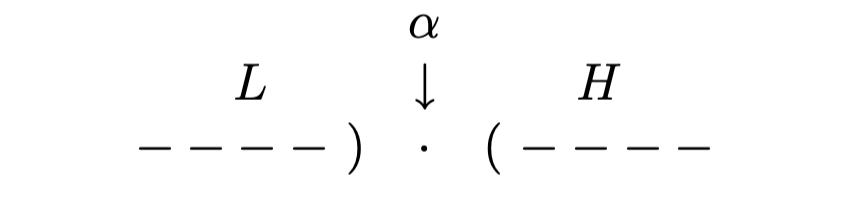
\includegraphics[scale=0.25]{CA.png}
    \caption{Completeness Axiom}
    \label{}
\end{figure}\end{center}

\begin{claim}
    \normalfont
    The Completeness Axiom differentiates $\mathbb{R}$ from $\mathbb{Q}$:\\
    $\mathbb{Q}$ satisfies all the axioms for $\mathbb{R}$ except the Completeness Axiom.
\end{claim}

\subsection{Supremum $\sup\mathbb{X}$, Infimum $\inf\mathbb{X}$ for $\mathbb{X}\subseteq \mathbb{R}$}
\begin{definition}[Supremum and Infimum]
    \normalfont
    \begin{enumerate}[(1).]
        \item Suppose $\mathbb{X}$ is bounded above. The \textbf{supremum} of $\mathbb{X}$, written $\sup\mathbb{X}$, is the least upper bound for $\mathbb{X}$, i.e. $\sup\mathbb{X}$ satisfies
        \begin{enumerate}
            \item $\sup\mathbb{X} \geq x,\forall x\in \mathbb{X}$ ($\sup\mathbb{X}$ is an upper bound).
            \item $\forall y<\sup\mathbb{X}$, $\exists x\in\mathbb{X}$ s.t. $x>y$ (there is no smaller upper bound).
        \end{enumerate}
        \item Suppose $\mathbb{X}$ is bounded below. The \textbf{infimum} of $\mathbb{X}$, written $\inf\mathbb{X}$, is the greatest lower bound for $\mathbb{X}$, i.e. $\inf\mathbb{X}$ satisfies
        \begin{enumerate}
            \item $\inf\mathbb{X} \leq x,\forall x\in \mathbb{X}$ ($\inf\mathbb{X}$ is a lower bound).
            \item $\forall y>\inf\mathbb{X}$, $\exists x\in\mathbb{X}$ s.t. $x<y$ (there is no greater lower bound).
        \end{enumerate}
        \item If $\mathbb{X}$ is not bounded above, write sup $\mathbb{X} = \infty$. If $\mathbb{X}$ is not bounded below, write inf $\mathbb{X} = -\infty$. By convention, $\sup \emptyset = -\infty$, $\inf \emptyset = +\infty$.
    \end{enumerate}
\end{definition}

\subsection{Theorem: $\sup/\inf$ in set is $\max/\min$}
\begin{proposition}[$\sup/\inf$ in set is $\max/\min$]
    If $\inf A=x^*\in A$ ($\sup A=x^*\in A$), then $x^*=\min A$ ($x^*=\max A$).
\end{proposition}

\subsection{Transformation of $\sup/\inf$}
\begin{theorem}
    Let $A$ and $B$ be nonempty sets of real numbers,
    \begin{enumerate}
        \item both of them bounded above, $\sup\{a+b:a\in A,b\in B\}=\sup A+\sup B$.
        \item bounded above and below respectively, $\sup\{a-b:a\in A,b\in B\}=\sup A-\inf B$
        \item $\inf A=-\sup(-A)$
    \end{enumerate}
\end{theorem}

\subsection{The Supremum Property: Nonempty set in $\mathbb{R}$ is bounded above/below $\Rightarrow$ $\exists \sup/\inf$}
\begin{proposition}[The Supremum Property]\label{The Supremum Property}
    \normalfont
    Every nonempty set of real numbers that is bounded above has a supremum, which is a real number. Every nonempty set of real numbers that is bounded below has an infimum, which is a real number.
\end{proposition}

\begin{theorem}
    The Supremum Property (Prop \ref{The Supremum Property}) and the Completeness Axiom (Prop \ref{Completeness Axiom}) are equivalent.
\end{theorem}

\subsection{Archimedean Property}
\begin{theorem}[Archimedean Property]
    $\forall x\in \mathbb{R}, y\in \mathbb{R}^+$, $\exists n\in \mathbb{N}$ s.t. $ny>x$.
\end{theorem}

\section{Metric Spaces and Normed Spaces \small{(@ Lec 03 of ECON 204)}}
\subsection{Metric Space $(\mathbb{X}, d)$ and Metric $d : \mathbb{X} \times \mathbb{X} \rightarrow \mathbb{R}_+$}
\begin{definition}[Metric Space]
\normalfont
    A \textbf{metric space} is a pair $(\mathbb{X}, d)$, where $\mathbb{X}$ is a set and $d : \mathbb{X} \times \mathbb{X} \rightarrow \mathbb{R}_+$ a function satisfying
    \begin{enumerate}
        \item Non-negative: $d(x,y)\geq 0$, $d(x,y)=0\Leftrightarrow x=y, \forall x,y\in \mathbb{X}$.
        \item Symmetric: $d(x,y)=d(y,x), \forall x,y\in \mathbb{X}$.
        \item Triangle inequality: $d(x,z)\leq d(x,y)+d(y,z), \forall x,y,z\in \mathbb{X}$.
    \end{enumerate}
    A function $d : \mathbb{X} \times \mathbb{X} \rightarrow \mathbb{R}_+$ satisfying 1-3 is called a \textbf{metric} on $\mathbb{X}$.
\end{definition}
A metric gives a notion of distance between elements of $\mathbb{X}$.

\subsection{Theorem: Subset forms a metric space}
\begin{theorem}[Subset forms a metric space]
    Given a metric space $(X, d)$, $(Y, d)$ for some $Y \subseteq X$ is still a metric space.
\end{theorem}

\subsection{Norm $\|\cdot\|$ and Normed Vector Space $(V,\|\cdot\|)$}
\begin{definition}[Norm]
\normalfont
    Let $V$ be a vector space over $\mathbb{R}$. A \textbf{norm} on $V$ is a function $\|\cdot\| : V \rightarrow \mathbb{R}_+$ satisfying
    \begin{enumerate}
        \item Non-negative: $\|x\|\geq 0$, $\|x\|=0\Leftrightarrow x=0, \forall x\in V$.
        \item Triangle inequality: $\|x+y\|\leq \|x\|+\|y\|, \forall x,y\in V$.
        \item $\|\alpha x\|=|\alpha|\|x\|$, $\forall \alpha\in \mathbb{R},x\in V$.
    \end{enumerate}
\end{definition}
A norm gives a notion of length of a vector in $V$.

\begin{definition}[Normed Vector Space]
\normalfont
    A \textbf{normed vector space} is a vector space over $\mathbb{R}$ equipped with a norm, $(V,\|\cdot\|)$.
\end{definition}
\begin{example}[ Normed Vector Space]
\begin{enumerate}[-]
    \item $\mathbf{E}^n: n$-dimensional Euclidean space.
    $$
    V=\mathbb{R}^n,\|x\|_2=|x|=\sqrt{\sum_{i=1}^n\left(x_i\right)^2}
    $$
    \item $V=\mathbb{R}^n,\|x\|_1=\sum_{i=1}^n\left|x_i\right|$ (the "taxi cab" norm or $L^1$ norm)
    \item $V=\mathbb{R}^n,\|x\|_{\infty}=\max \left\{\left|x_1\right|, \ldots,\left|x_n\right|\right\}$ (the maximum norm, or sup norm, or $L^{\infty}$ norm)
    \item $C([0,1]),\|f\|_{\infty}=\sup \{|f(t)|: t \in[0,1]\}$
    \item $C([0,1]),\|f\|_2=\sqrt{\int_0^1(f(t))^2 d t}$
    \item $C([0,1]),\|f\|_1=\int_0^1|f(t)| d t$
\end{enumerate}
where $C([0,1])$ is the space of all continuous real-valued functions on $[0,1]$.
\end{example}

\subsection{Subset may not form a normed vector space}
Given a normed vector space $(V, \|\cdot\|)$, is $(W, \|\cdot\|)$ for some $W \subseteq V$, $W$ may not be a vector space (e.g. it may not contain the zero vector)!

\subsection{Theorem: metric can be defined by norm}
In an abstract normed vector space, the norm can be used analogously to define a notion of distance.
\begin{theorem}[Metric can be defined by norm]
    Let $(V,\|\cdot\|)$ be a normed vector space. Let $d : \mathbb{X} \times \mathbb{X} \rightarrow \mathbb{R}_+$ be defined by $d(v, w) = \|v-w\|$. Then $(V, d)$ is a metric space.
\end{theorem}

\subsection{Cauchy-Schwarz Inequality}
\begin{theorem}[Cauchy-Schwarz Inequality]
    If $v, w \in \mathbb{R}^n$, then
    $$
    \begin{aligned}
    \left(\sum_{i=1}^n v_i w_i\right)^2 & \leq\left(\sum_{i=1}^n v_i^2\right)\left(\sum_{i=1}^n w_i^2\right) \\
    \|v \cdot w\|^2 & \leq\|v\|^2\|w\|^2 \\
    \|v \cdot w\| & \leq\|v\|\|w\|
    \end{aligned}
    $$
\end{theorem}

\subsection{Lipschitz-equivalent Norm}
\begin{definition}[Lipschitz-equivalent]
\normalfont
Two norms $\|\cdot\|$ and $\|\cdot\|^*$ on the same vector space $V$ are said to be \textbf{Lipschitz-equivalent} (or \textbf{equivalent}) if $\exists m,M>0$ s.t. $\forall x\in V$, $$m\|x\|\leq\|x\|^*\leq M\|x\|$$
Equivalently, $\exists m,M>0$ s.t. $\forall x\in V$, $x\neq 0$, $$m\leq\frac{\|x\|^*}{\|x\|}\leq M$$
\end{definition}
\begin{theorem}
    All norms on $\mathbb{R}^n$ are equivalent.
\end{theorem}
However, infinite-dimensional spaces support norms that are not equivalent. For example, on $C([0, 1])$, let $f_n$ be the function $$f_n(t)=\left\{\begin{matrix}
    1-nt,&\textnormal{if }t\in[0,\frac{1}{n}]\\
    0,&\textnormal{if }t\in(\frac{1}{n},1]
\end{matrix}\right.$$ Then $\frac{\|f_n\|_1}{\|f_n\|_\infty}=\frac{1}{2n}\rightarrow 0$, which means there is no lower bound $m>0$.

\subsection{Ball, Radius, Diameter, and Distance}
In a metric space $(X, d)$, define
$$
\begin{aligned}
B_{\varepsilon}(x) & =\{y \in X: d(y, x)<\varepsilon\} \\
& =\text { open ball with center } x \text { and radius } \varepsilon \\
B_{\varepsilon}[x] & =\{y \in X: d(y, x) \leq \varepsilon\} \\
& =\text { closed ball with center } x \text { and radius } \varepsilon
\end{aligned}
$$
We can use the metric $d$ to define a generalization of "radius". In a metric space $(X, d)$, define the \textit{diameter} of a subset $S \subseteq X$ by
$$
\operatorname{diam}(S)=\sup \left\{d\left(s, s^{\prime}\right): s, s^{\prime} \in S\right\}
$$
Similarly, we can define the \textit{distance from a point to a set}, and \textit{distance between sets}, as follows:
$$
\begin{aligned}
d(A, x) & =\inf _{a \in A} d(a, x) \\
d(A, B) & =\inf _{a \in A} d(B, a) \\
& =\inf \{d(a, b): a \in A, b \in B\}
\end{aligned}
$$

\section{Set Theory}
\subsection{Well Defined Set}
\begin{definition}
    A set $S$ is \textbf{well defined} if an object $a$ is either $a\in S$ or $a\notin S$.
\end{definition}

\subsection{Numerically Equivalent: $\exists$ bijection \small{(@ Lec 01 of ECON 204)}}
\begin{definition}
\normalfont
    Two sets $A, B$ are \textbf{numerically equivalent} (or have the same cardinality) if there is a bijection $f : A \rightarrow B$, that is, 1-1 ($a \neq a' \Rightarrow f(a) \neq f(a')$), and onto ($\forall b\in B, \exists a\in A$ s.t. $f(a)=b$).
\end{definition}

\subsection{Finite \small{(@ Lec 01 of ECON 204)}}
\begin{definition}[Finite Set]
\normalfont
    A set is either \textbf{finite} or \textbf{infinite}. A set is \textbf{finite} if it is \underline{numerically equivalent to} $\{1,...,n\}$ for some $n$. A set that is not finite is infinite.
\end{definition}

\subsection{Countable Set: numerically equivalent to $\mathbb{N}$ \small{(@ Lec 01 of ECON 204)}}
We give a more precise definition to classify infinite set:
\begin{definition}[Countable Set]
\normalfont
    An infinite set is \textbf{countable} if it is \underline{numerically equivalent to} $\mathbb{N}$. An infinite set that is not countable is called \textbf{uncountable}.
\end{definition}

\begin{theorem}[Countable $\mathbb{Q}$]
    The set of rational numbers $\mathbb{Q}$ is countable.
\end{theorem}


\subsection{Power Set \small{(@ Lec 02 of ECON 204)}}
\begin{definition}[Power Set: the set of all subsets]
    For any set $A$, we denote by $\mathcal{P}(A)$ the collection of all subsets of $A$. $\mathcal{P}(A)$ is the \textbf{power set} of $A$.
\end{definition}
We may also use the notation $2^A$ (in Berkeley ECON 204).

\subsection{Theorem (Cantor): The power set of $\mathbb{N}$ is uncountable \small{(@ Lec 02 of ECON 204)}}
\begin{theorem}[Cantor]
    $\mathcal{P}(\mathbb{N})$ (or denoted by $2^\mathbb{N}$), the set of all subsets of $\mathbb{N}$, is uncountable.
\end{theorem}

\subsection{Cardinalities of Sets \small{(@ Lec 02 of ECON 204)}}
\begin{definition}[Cardinality]
    If $A$ is a set, $|A|=$ cardinality of $A$ = $\#$ of elements
\end{definition}
$n \in \mathbb{N},|\{1, \ldots n\}|=n$; $|\emptyset|=0(\emptyset=\text { empty set })$.

\begin{proposition}[Facts about cardinality]
    \begin{enumerate}
        \item If $A$ is numerically equivalent to $\{1,...,n\}$ for some $n\in \mathbb{N}$, then $|A|=n$.
        \item $A$ and $B$ are numerically equivalent if and only if $|A|=|B|$.
        \item If $|A| = n$ (finite) and $A$ is a proper subset of $B$ (that is, $A\subset B$ and $A \neq B$) then $|A|<|B|$.
        \item If $A$ is countable and $B$ is uncountable, then $n<|A|<|B|, \forall n\in\mathbb{N}$.
        \item If $A\subseteq B$, then $|A|\leq|B|$. (if $B$ is countable and $A\subseteq B$, then $A$ is at most countable, that is, $A$ is either empty, finite, or countable.)
        \item If there is an \textit{injection} $\sigma:A \rightarrow B$, we can write $|A|\leq|B|$;
        \item If there is a \textit{surjection} $\sigma:A \rightarrow B$, we can write $|A|\geq|B|$;
        \item If there is a bijection $\sigma:A \rightarrow B$, we can write $|A|=|B|$.
    \end{enumerate}
\end{proposition}

\subsection{Pigeonhole Principle: $|A|>|B|$ $\Rightarrow$ no injective function $\sigma:A \rightarrow B$}
\begin{theorem}[Pigeonhole Principle]
    If $A$ and $B$ are sets and $|A|>|B|$, then there is no injective function $\sigma:A \rightarrow B$.
\end{theorem}



\subsection{$B^A$: Sets of Function}
If $A,B$ are sets, then $B^A=\{\sigma:A \rightarrow B| \sigma \textit{ a function}\}$.
\begin{example}
    $n\in \mathbb{Z}$, we define a function $f: B^{\{1,\dots,n\}} \rightarrow B^n(=B\times B\times B\times \dots \times B)$ by the equation
    $f(\sigma)=\{\sigma(1),...,\sigma(n)\}, \textit{ where }\sigma:\{1,\dots,n\} \rightarrow B$. The $f$ is a \textit{bijection}.
\end{example}
\begin{proof}
    \quad\\
    1. \textit{Injective}:
    \begin{equation}
        \begin{aligned}
            &f(\sigma_1)=f(\sigma_2)
            \Rightarrow \{\sigma_1(1),...,\sigma_1(n)\}=\{\sigma_2(1),...,\sigma_2(n)\}\\
            &\textit{Since }\sigma:\{1,\dots,n\} \rightarrow B,\textit{ it is sufficient to prove }\sigma_1=\sigma_2.
        \end{aligned}
        \nonumber
    \end{equation}
    2. \textit{Surjective}:
    \begin{equation}
        \begin{aligned}
            &\forall \{b_1,...,b_n\},\textit{ we have }\sigma^*(x)=b_x,x=1,...,n.\textit{ s.t. }f(\sigma^*)=\{b_1,...,b_n\}
        \end{aligned}
        \nonumber
    \end{equation}

\end{proof}
\begin{example}
    \begin{equation}
        \begin{aligned}
            & C(\mathbb{R},\mathbb{R})=\{\textit{continuous functions }\sigma:\mathbb{R} \rightarrow \mathbb{R} \}\subset \mathbb{R}^\mathbb{R}
        \end{aligned}
        \nonumber
    \end{equation}
\end{example}



\subsection{Bounded Set \small{(@ Lec 03 of ECON 204)}}
\begin{definition}[Bounded Set]
    \normalfont
    In a metric space $(X, d)$, a subset $S \subseteq X$ is \textbf{bounded} if $\exists x \in X, \beta \in \mathbb{R}$ such that $\forall s \in S$, $d(s, x) \leq \beta$.
\end{definition}
Equivalent: $\exists \beta>0$ and $s\in S$ such that $S\subseteq B_\beta(s)$.



\subsection{Open, Closed Set \small{(@ Lec 04 of ECON 204)}}
\begin{definition}[Open Sets]
    Let $(X, d)$ be a metric space. A set $\mathbb{X} \subseteq \mathbb{R}^{n}$ is \textbf{open} if
    
    $\forall x \in \mathbb{X}$ we can draw a ball around $x$ that is contained in $\mathbb{X}$.

    i.e. $\forall x \in \mathbb{X}, \exists \varepsilon>0$ s.t. $B_\varepsilon(x)=\{y:d(y,x)<\varepsilon\} \subseteq \mathbb{X}$
\end{definition}

\begin{example}
    In a metric space $(X, d)$, if $a$ is an isolated point of $X$, then the singleton set $\{a\}$ is open: Since $a$ is not a limit point of $X$, we can find a neighborhood $B_\varepsilon(a)$ such that $B_\varepsilon(a)\cap X = \{a\}$. So $B_\varepsilon(a) \subseteq \{a\}$ and $x$ is an interior point. Hence, every point is an interior point and the set is open.
\end{example}

\begin{definition}[Closed Sets]
    $\mathbb{X}$ is \textbf{closed} if $\mathbb{X}^c$ is open.
\end{definition}
\begin{theorem}[Equivalent definition: Closed Sets]
    Equivalent: if $A$ in a metric space $(X, d)$ contains all limit points of all sequences in $A$, $A$ is closed.
    $$\{x_n\}\subset A, x_n \rightarrow x\in X \Rightarrow x\in A$$
\end{theorem}
\begin{example}[ (Closed and Open Sets on $\mathbb{E}_1$ i.e., $\mathbb{R}$ with the usual Euclidean metric)]
\end{example}
\begin{enumerate}[1)]
    \item $(1,2)=\{x \in \mathbb{R}: 1<x<2\}$ - open
    \item $\mathbb{R}$ is both open and closed
    \item $(-\infty, 1)=\{x \in \mathbb{R}: x<1\}$ - open
    \item $[1, \infty)$ is closed because its complement open
    \item $(1,2]$ is neither open nor closed
\end{enumerate}

\begin{example}[ (Closed and Open Sets on other metric space)]
    In the metric space $[0, 1]$, $[0, 1]$ is open. With $[0, 1]$ as the underlying metric space, $B_\varepsilon(0) = \{x \in [0, 1] : |x - 0| < \varepsilon\} = [0,\varepsilon)$.
\end{example}

\begin{theorem}
    [Empty Set and Full Set are both open and closed]
    In any metric space $(X, d)$ both $\emptyset$ and $X$ are open, and both $\emptyset$ and $X$ are closed.
\end{theorem}

\begin{theorem}[Every neighborhood is an open set]
    Every neighborhood $B_\varepsilon(x)$ is an open set.
\end{theorem}

\begin{theorem}[Finite sets are closed in any metric space]
    Finite sets are closed in any metric space $(X, d)$.
\end{theorem}

\begin{proposition}
    Any set in a metric space $(X, d)$ can be written as the intersection of open sets.
\end{proposition}

\subsection{$\bigstar$ Theorem: Union of open sets is open, Intersection of finite open sets is open}
\begin{theorem}[Union of open sets is open, Intersection of finite open sets is open]
    In any metric space $(X, d)$,
    \begin{enumerate}
        \item The union of an arbitrary (finite, countable, or uncountable) collection of open sets is open.
        \item The intersection of a finite collection of open sets is open.
    \end{enumerate}
\end{theorem}

\subsection{$\bigstar$ Corollary: Intersection of closed sets is closed, Union of finite closed sets is closed}
\begin{corollary}[Intersection of closed sets is closed, Union of finite closed sets is closed]
    In any metric space $(X, d)$,
    \begin{enumerate}
        \item The intersection of an arbitrary collection of closed sets is closed.
        \item The union of a finite collection of closed sets is closed.
    \end{enumerate}
\end{corollary}

\subsection{Interior, Exterior, Boundary, Closure \small{(@ Lec 04 of ECON 204)}}
Given a set $S\subseteq X$, the \textbf{point} of $X$ can be classified into three types relative to $S$:
\begin{enumerate}[$\bullet$]
    \item \textbf{Interior (points)}, denoted $int(S)$: $\vec{x}\in S$ for which there exists some $B(\vec{x},r)\subseteq S$, is the largest open set contained in $S$ (the union of all open sets contained in $S$). $$x\in \textnormal{int }A \Leftrightarrow \exists \varepsilon>0: B_\varepsilon(x)\subseteq A$$
    \item \textbf{Exterior (points)}, denoted $ext(S)$: $\vec{x}\notin S$ for which there exists some $B(\vec{x},r)$ containing \underline{no} points of $S$, is the largest open set contained in $X \backslash S$.
    $$x\in \textnormal{ext }A \Leftrightarrow \exists \varepsilon>0: B_\varepsilon(x)\subseteq A^C$$
    \item \textbf{Boundary (points)} denoted $\partial (S)$ or $bd(S)$: all other points (for which any $B(\vec{x},r)$ will contain some points of $S$ and some points outside $S$).
    $$x\in \partial A \Leftrightarrow \forall \varepsilon>0: B_\varepsilon(x)\cap A\neq\emptyset \textnormal{ and } B_\varepsilon(x)\cap A^C\neq\emptyset$$
    \item \textbf{Closure of $S$}, denoted $\bar{S}$ or $cl(S)=int(S)\cup \partial(S)$,  is the smallest closed set containing $S$ (the intersection of all closed sets containing $S$).
    $$x\in \textnormal{cl }A \Leftrightarrow \forall \varepsilon>0: B_\varepsilon(x)\cap A\neq\emptyset$$
    \item Moreover, boundary satisfies $\partial (S)=\overline{(X\backslash S)}\cap\bar{S}$.
\end{enumerate}

\begin{proposition}
    \begin{enumerate}[(1)]
        \item $int A$, $ext A$ and $\partial A$ partition $X$.
        \item $int A$ and $\partial A$ partition $cl A$.
        \item A set $S$ is \textbf{open} iff $S=int(S)$ - i.e., $S$ does \underline{not} contain any of its boundary points.
        \item A set $S$ is \textbf{closed} iff $S=\bar{S}=int(S)\cup \partial(S)$ - i.e., $S$ contains \underline{all} of its boundary points.
        \item A set $S$ is \textbf{open} and \textbf{closed} iff $\partial(S)=\emptyset$.
        \item $\overline{A\cap B}\subseteq \bar{A}\cap\bar{B}$.
    \end{enumerate}
\end{proposition}

\subsection{Dense Set: $\bar{A}=X$}
\begin{definition}[Dense Set]
    \normalfont
    Let $(X,d)$ be a metric space. A set $A\subseteq X$ is \textbf{dense} in $X$ if $\bar{A}=X$.
\end{definition}
\begin{example}
    $\mathbb{Q}$ is dense in $\mathbb{R}$: for all $x\in \mathbb{Q}$, let $y_n=\frac{\lfloor 10^nx\rfloor}{10^n}$ with $n\in \mathbb{N}$. Then, $\{y_n\}\subseteq \mathbb{Q}$, and $y_n \rightarrow x$ since $|y_n-x|<10^{-n}$. Then $\exists N\in \mathbb{N}$ s.t. $\forall n> N$, $|y_n-x|<\varepsilon$ (or $y_n\in B_{\varepsilon}(x)$). This implies $B_\varepsilon(x)\cap \mathbb{Q}\neq \emptyset$, so $\bar{\mathbb{Q}}=\mathbb{R}$.
\end{example}
\begin{corollary}[$\mathbb{Q}^n$ is dense in $\mathbb{R}^n$]
    $\mathbb{Q}^n$ is dense in $\mathbb{R}^n$ for $n\in \mathbb{N}$.
\end{corollary}

\begin{theorem}
    If $A$ is dense in $X$, for all $x\in X$: $\forall \varepsilon>0, B_\varepsilon(x)\cap A\neq \emptyset$.
\end{theorem}
\begin{proof}
    Since $A$ is dense in $X$, then for any $x\in X=\bar{A}$, $\forall \varepsilon>0, B_\varepsilon(x)\cap A\neq \emptyset$ by the definition of closure.
\end{proof}

\begin{example}
    If $\mathcal{A}$ is a collection of open subsets of $\mathbb{R}^n$, pairwise disjoint, that is, $A_\lambda \cap A_{\lambda'} = \emptyset$ if $\lambda\neq\lambda'$, then $\mathcal{A}$ is at most countable.
\end{example}
Let $\Lambda$ be the set of indices of $\mathcal{A}$, i.e., $\mathcal{A}=\{A_\lambda\}_{\lambda\in\Lambda}$. Choose an arbitrary $\lambda\in\Lambda$, and choose an arbitrary point $x\in A_\lambda$. Since $A_\lambda$ is open, $\exists \varepsilon>0$ s.t. $B_\varepsilon(x)\subseteq A_\lambda$. Because $\mathbb{Q}^n$ is dense in $\mathbb{R}^n$, $\exists q_\lambda\in \mathbb{Q}^n$ s.t. $q_\lambda\in B_\varepsilon(x)\subseteq A_\lambda$. Therefore, $\forall \lambda\in\Lambda$, $\exists q_\lambda\in \mathbb{Q}^n$ s.t. $q_\lambda\in B_\varepsilon(x)\subseteq A_\lambda$. Therefore, $\forall \lambda\in \Lambda$, $\exists q_\lambda\in \mathbb{Q}^n$ s.t. $q_\lambda\in A_\lambda$. Note that $\mathcal{A}$ is a collection of pairwise disjoint open sets, then $\forall \lambda,\lambda'\in\Lambda$, $\lambda\neq\lambda'$, $q_\lambda\neq q'_\lambda$. Therefore, we can consider a function $f: \mathcal{A} \rightarrow \mathbb{Q}^n$, with $f(A_\lambda)=q_\lambda, \forall \lambda\in\Lambda$. Since $\forall \lambda,\lambda'\in\Lambda, \lambda\neq\lambda',q_\lambda\neq q'_\lambda$, then $f$ is an injection. This indicates the cardinality of $\mathbb{Q}^n$ is weakly larger than $\mathcal{A}$, then $\mathcal{A}$ is at most countable.


\subsection{Compact Set}
\begin{definition}[Compact Set]
    \normalfont
    $\mathbb{X} \subseteq \mathbb{R}^{n}$ is compact of it is closed and bounded.
\end{definition}

\begin{example}[ Compact Set]
    \normalfont
    $[1,2]=\{x \in \mathbb{R}: 1 \leqslant x \leqslant 2\}$; $\left\{x \in \mathbb{R}^{2}\right.: \left.x_{1}^{2}+x_{2}^{2} \leqslant 4\right\}$
\end{example}

\subsection{Sublevel Set}
\begin{definition}[Sublevel Set]
    \normalfont
    The sublevel set of a function $f: \mathbb{R}^n \rightarrow \mathbb{R}$ (for some level $c\in \mathbb{R}$) is the set $$\overline{L_c}=\{x\in \mathbb{R}^n:f(x)\leq c\}$$
\end{definition}



\subsection{Set Operations}
\begin{definition}
    \normalfont
    A \underline{binary operation} on a set $A$ is a function $*:A\times A \rightarrow A$.\\
    The \underline{operation is \textit{associative}} if $a*(b*c)=(a*b)*c, \forall a,b,c\in A$.\\
    The \underline{operation is \textit{commutative}} if $a*b=b*a, \forall a,b\in A$.
\end{definition}

\begin{example}

${+,\circ}$ are both \textit{associative} and \textit{commutative} operations on $\mathbb{Z},\mathbb{N},\mathbb{Q},\mathbb{R}$; $-$ is a neither \textit{associative} nor \textit{commutative} operation on $\mathbb{Z},\mathbb{Q},\mathbb{R}$, but not $\mathbb{N}$.
\end{example}

\begin{definition}
A subset $H\subset S$ is \underline{closed under $*$} if $a*b\in H$ for all $a,b\in H$.
\end{definition}

\begin{definition}
$*$ has \underline{identity element $e\in S$} if $a*e=e*a=a$ for all $s\in S$.
\end{definition}

\subsection{Connected Sets \small{(@ Lec 07 of ECON 204)}}
\begin{definition}[Separated/Connected Set]
    \normalfont
    Two sets $A, B$ in a metric space are \textbf{separated} if $$\bar{A}\cap B=A\cap\bar{B}=\emptyset$$
    where $\bar{A}$ is the closure of $A$.

    A set in a metric space is \textbf{connected} if it cannot be written as the union of two nonempty separated sets.
\end{definition}
\textbf{Equivalent Definition:} A set $Y$ in a metric space $X$ is connected if there do not exist \textit{open sets} $A$ and $B$ such that $A \cap B = \emptyset$, $Y \subseteq A\cup B$ and $A \cap Y \neq \emptyset$ and $B \cap Y \neq \emptyset$.

\textbf{Note} that separation does not require that $\bar{A}\cap\bar{B}=\emptyset$. For example, $[0,1)\cup(1,2]$ is not connected, since $[0,1)$ and $(1,2]$ are separated.

\subsection{Theorem: Connected Set over $\mathbb{E}^1$ $\Leftrightarrow$ Interval \small{(@ Lec 07 of ECON 204)}}
\begin{theorem}[Connected Set over $\mathbb{E}^1$ $\Leftrightarrow$ Interval]
    A set $S \subseteq \mathbb{E}^1$ of real numbers is \textbf{connected} \underline{if and only if} it is an \textbf{interval}, i.e. if $x, y \in S$ and $z \in (x, y)$, then $z \in S$.
\end{theorem}
Notice that this result is only valid in $\mathbb{R}$. For example, connected sets in $\mathbb{R}^n$ need not be intervals, or even convex.

\subsection{Theorem: Continuous Image of Connected Set is Connected}
\begin{theorem}[Continuous Image of Connected Set is Connected]
    Let $X$ be a metric space and $f : X \rightarrow Y$ be continuous. If $C$ is a connected subset of $X$, then $f(C)$ is connected.
\end{theorem}

\subsection{Intermediate Value Theorem proved by connectedness}
\begin{corollary}[Intermediate Value Theorem]
    If $f : [a, b] \rightarrow \mathbb{R}$ is continuous, and $f(a) < d < f(b)$, then there exists $c \in (a, b)$ such that $f(c) = d$.
\end{corollary}
\begin{proof}
    Since $[a, b]$ is an interval, it is connected. So $f([a, b])$ is connected, hence $f([a, b])$ is an interval. $f(a) \in f([a, b])$, and $f(b) \in f([a, b])$, and $d \in [f(a), f(b)]$; since $f([a, b])$ is an interval, $d \in f([a, b])$, i.e. there exists $c \in [a, b]$ such that $f(c) = d$. Since $f(a) < d < f(b)$, $c \neq a, c \neq b$, so $c \in (a, b)$.
\end{proof}


\section{Sequences}
Sequences $\left\{x_{k}\right\}_{k=1}, \ldots$ or $\left\{x_{k}\right\}, x_{k} \in \mathbb{R}^{n}$

\begin{definition}[Subsequence]
\normalfont
    Suppose $\{x_n\}$ is a sequence and $n_1<n_2<\cdots$, then $\{x_{n_k}\}$ is called a \textbf{subsequence}.
\end{definition}

\subsection{Convergence of Sequences \small{(@ Lec 03 of ECON 204)}}
\begin{definition}[Convergence: note $x_{k} \rightarrow x, \lim _{k \rightarrow \infty} x_{k}=x$]
    Let $(X, d)$ be a metric space. A sequence $\{x_k\}$ converges to $x$ (written $x_{k} \rightarrow x$ or $\lim _{k \rightarrow \infty} x_{k}=x$) if $\forall \varepsilon>0, \exists N_{\varepsilon}$ s.t. $d(x_{k},x)<\varepsilon,\ \forall k \geqslant N_{\varepsilon}$
\end{definition}

\subsection{Limit Point \small{(@ Lec 03 of ECON 204)}}
\begin{definition}[Limit Point]
    \normalfont $x$ is a \textbf{limit point} of $\left\{x_{k}\right\}$ if $\exists \text { a subsequence of }\left\{x_{k}\right\} \text { that converges to } x$.
\end{definition}

\begin{definition}[Limit Point, alternative definition]
    \normalfont
    Let $(X,d)$ be a metric space. A point $x\in X$ is a \textbf{limit point} of a set $A\subseteq X$ if $$\forall \varepsilon>0, B_\varepsilon(x)\cap A\nsubseteq\{x\}$$
\end{definition}

\begin{theorem}[Set of limit points of any set $A\subseteq \mathbb{R}^n$ is closed.]
    The set of limit points of any set $A\subseteq \mathbb{R}^n$ is closed.
\end{theorem}
\begin{proof}
    Suppose $\mathcal{S}$ is the set of limit points of $A$. Let $D=\mathbb{R}^n\backslash \mathcal{S}$. Take an arbitrary $x\in D$. Then $x$ is not the limit point of $A$, so $\exists\varepsilon_x>0$ s.t. $B_{\varepsilon_x}(x)\cap A\subseteq\{x\}$. For any $y\in B_{\varepsilon_x}(x)$, since $B_{\varepsilon_x}(x)$ is open, $\exists \varepsilon_y>0$ s.t. $B_{\varepsilon_y}(y)\subseteq B_{\varepsilon_x}(x)$. Let $\varepsilon_m=\min\{d(x,y),\varepsilon_y\}$ such that $B_{\varepsilon_m}(y)\subseteq B_{\varepsilon_x}(x)$ and $x\notin B_{\varepsilon_m}(y)$. So, $B_{\varepsilon_m}(y)\cap A=\emptyset$. So, $y$ is not a limit point of $A$, that is $y\in \mathbb{R}^n\backslash \mathcal{S}=D$. Therefore, $\forall y\in B_{\varepsilon_x}(x) \Rightarrow y\in D$. We can conclude $B_{\varepsilon_x}(x)\subseteq D, \forall x\in D$. So, $D$ is open.
\end{proof}

\begin{theorem}[Subsequence has the same limit as the original sequence]
    All subsequences of a convergent sequence converge to the same limit as the original sequence.
\end{theorem}

\begin{theorem}[Uniqueness of Limits]
    In a metric space $(X, d)$, if $x_{k} \rightarrow x$ and $x_{k} \rightarrow x'$, then $x=x'$.
\end{theorem}

\subsection{Cluster Point \small{(@ Lec 03 of ECON 204)}}
\begin{definition}[Cluster Point]
\normalfont
    An element $c$ is a \textbf{cluster point} of a sequence $\{x_n\}$ in a metric space $(X, d)$ if $\forall\varepsilon > 0, \{n : x_n \in B_\varepsilon(c)\}$ is an infinite set. Equivalently, $$\forall\varepsilon > 0, N\in \mathbb{N}, \exists n>N \textnormal{ s.t. } x_n \in B_\varepsilon(c)$$
\end{definition}
\begin{example}
    $x_n=\left\{\begin{matrix}
        1-\frac{1}{n},& \textnormal{ if $n$ even}\\
        \frac{1}{n},&\textnormal{ if $n$ odd}
    \end{matrix}\right.$ has cluster points $\{0,1\}$.
\end{example}

\begin{theorem}[Cluster Point $\Leftrightarrow$ exists subsequence converges to it]
    Let $(X, d)$ be a metric space, $c \in X$, and $\{x_n\}$ a sequence in $X$. Then $c$ is a cluster point of $\{x_n\}$ if and only if there is a subsequence $\{x_{n_k}\}$ such that $\lim_{k \rightarrow \infty} x_{n_k} = c$.
\end{theorem}

\subsection{Proposition: Sequences in $\mathbb{R}^n$, Bounded above and non-decreasing sequence $\Rightarrow$ Converge}
\begin{proposition}
    If $\left\{x_{k}\right\}$ is bounded above(below) and non-decreasing(non-increasing) it \textbf{converges}.
\end{proposition}

\subsection{Theorem: Increasing/Decreasing Sequences in $\mathbb{R}^n$, Limit is $\sup$/$\inf$ \small{(@ Lec 03 of ECON 204)}}

\begin{theorem}
    Let $\{x_n\}$ be an increasing (decreasing) sequence of real numbers. Then $\lim_{n \rightarrow \infty} x_n = \sup\{x_n : n \in \mathbb{N}\}$ ($\lim_{n \rightarrow \infty} x_n = \inf\{x_n : n \in \mathbb{N}\}$). In particular, the limit exists.
\end{theorem}

\subsection{Definition: $\lim\sup$ and $\lim\inf$ \small{(@ Lec 03 of ECON 204)}}
Consider a sequence $\{x_n\}$ of real numbers. Let $$\alpha_n=\sup\{x_k:k\geq n\}$$ and $$\beta_n=\inf\{x_k:k\geq n\}$$
Either $\alpha_n = +\infty$ for all $n$, or $\alpha_n \in \mathbb{R}$ and $\alpha_1 \geq \alpha_2 \geq \alpha_3 \geq...$. Either $\beta_n = -\infty$ for all n, or $\beta_n \in \mathbb{R}$ and $\beta_1 \leq \beta_2 \leq \beta_3 \leq ...$.
\begin{definition}[Lim Sups and Lim Infs]
    \normalfont
    $$
    \begin{aligned}
    & \limsup _{n \rightarrow \infty} x_n=\left\{\begin{array}{cl}
    +\infty & \text { if } \alpha_n=+\infty \text { for all } n \\
    \lim \alpha_n & \text { otherwise. }
    \end{array}\right. \\
    & \liminf _{n \rightarrow \infty} x_n=\left\{\begin{array}{cl}
    -\infty & \text { if } \beta_n=-\infty \text { for all } n \\
    \lim \beta_n & \text { otherwise. }
    \end{array}\right.
    \end{aligned}
    $$
\end{definition}

\subsection{Exists Limit $\Leftrightarrow$ $\lim=\lim\sup=\lim\inf$ \small{(@ Lec 03 of ECON 204)}}
\begin{theorem}
    Let $\left\{x_n\right\}$ be a sequence of real numbers. Then
    $$
    \begin{aligned}
    & \lim _{n \rightarrow \infty} x_n=\gamma \in \mathbb{R} \cup\{-\infty, \infty\} \\
    \Leftrightarrow & \lim \sup _{n \rightarrow \infty} x_n=\liminf _{n \rightarrow \infty} x_n=\gamma
    \end{aligned}
    $$
\end{theorem}

\subsection{Rising Sun Lemma: Sequence in $\mathbb{R}^n$ contains monotone subsequence \small{(@ Lec 03 of ECON 204)}}
\begin{theorem}[Rising Sun Lemma]
    Every sequence of real numbers contains an increasing subsequence or a decreasing subsequence or both.
\end{theorem}

\subsection{Bolzano-Weierstrass: Bounded Sequence in $\mathbb{R}^n$ contains a convergent subsequence \small{(@ Lec 03 of ECON 204)}}\label{B-W}
\begin{theorem}[Bolzano-Weierstrass]
    Every bounded sequence of real numbers contains a convergent subsequence.
\end{theorem}



\section{Complete Metric Spaces \small{(@ Lec 05 of ECON 204)}}
Roughly, a metric space is complete if “every sequence that ought to converge to a limit has a limit to converge to.”
\subsection{Cauchy Sequence}
\begin{definition}[Cauchy Sequence]
    A sequence $\{x_k\}$ in a metric space (X, d) is \textbf{Cauchy} if $\forall \varepsilon>0, \exists N(\varepsilon)$ s.t.
    $$d(x_{n},x_{m})<\varepsilon,\  \forall n, m > N(\varepsilon)$$
\end{definition}
\textbf{Note:} Cauchy property depends only on the sequence and the metric d, not on the ambient metric space.

\textbf{Note:} In $\mathbb{E}^1=(\mathbb{R},\|\cdot\|)$, $\left\{x_{k}\right\} \text { converges } \Longleftrightarrow\left\{x_{k}\right\} \text { is Cauchy}$.

A Cauchy sequence is trying really hard to converge, but there may not be anything for it to converge to. Any sequence that does converge must be Cauchy, however, by the argument above.

\subsection{Theorem: Convergent $\Rightarrow$ Cauchy}
\begin{theorem}[Convergent $\Rightarrow$ Cauchy]
    Every convergent sequence in a metric space is Cauchy.
\end{theorem}


\subsection{Complete Metric Space and Banach Space}
\begin{definition}[Complete Metric Spaces]
    \normalfont
    A metric space $(X, d)$ is \textbf{complete} if every Cauchy sequence $\{x_n\} \subseteq X$ converges to a limit $x \in X$.
\end{definition}
\begin{example}
    \begin{enumerate}
        \item Consider the earlier example of $X = (0, 1]$ with d the usual Euclidean metric. Since $x_n = \frac{1}{n}$ is Cauchy but does not converge in that metric space, $((0, 1], d)$ is not complete.
        \item $\mathbb{Q}$ is not complete in the Euclidean metric: $x_n=\frac{\left\lfloor 10^n \sqrt{2} \right\rfloor }{10^n} \rightarrow \sqrt{2}$.
    \end{enumerate}
\end{example}

\begin{definition}[Banach Space]
    \normalfont
    A \textbf{Banach space} is \textit{a normed space} that is complete in the metric generated by its norm.
\end{definition}

\begin{theorem}[$\mathbb{E}^1$ is complete]
    $\mathbb{R}$ is complete with the usual metric (so $\mathbb{E}^1$ is a Banach space).
\end{theorem}

\begin{theorem}[$\mathbb{E}^n$ is complete]
    $\mathbb{E}^n$ is complete for every $n \in \mathbb{N}$.
\end{theorem}

\begin{theorem}[$(C(X),\|\cdot\|_\infty)$ is Complete]
    Given $X \subseteq \mathbb{R}^n$, let $C(X)$ be the set of bounded continuous
    functions from $X$ to $R$ with $$\|f\|_\infty=\sup\{|f(x)|:x\in X\}$$
    Then $C(X)$ is a Banach space.
\end{theorem}

\subsection{$\bigstar$ Theorem: Subset of Complete Metric Space "is Complete" $\Leftrightarrow$ "is Closed"}
\begin{theorem}[Subset of Complete Metric Space "is Complete" $\Leftrightarrow$ "is Closed"]\label{complete_equal_closed}
    Suppose $(X, d)$ is a complete metric space and $Y \subseteq X$. Then $(Y, d) = (Y, d\mid_Y)$ is complete \underline{if and only if} $Y$ is a \textit{closed subset} of $X$. (where $d: \mathbb{X}\times \mathbb{X}\rightarrow \mathbb{R}_+$; $d\mid_Y: \mathbb{Y}\times \mathbb{Y}\rightarrow \mathbb{R}_+$)
\end{theorem}


\section{Compactness over Metric Spaces \small{(@ Lec 06 of ECON 204)}}
\subsection{Open Cover}
\begin{definition}[Open Cover]
    \normalfont
    A collection of sets $\mathcal{U} = \{U_\lambda : \lambda \in \Lambda\}$ in a metric space $(X, d)$ is an \textbf{open cover} of $A\subseteq X$ if
    \begin{enumerate}
        \item $U_\lambda$ is open for all $\lambda \in \Lambda$ and
        \item $A\subseteq \cup_{\lambda\in\Lambda}U_\lambda$
    \end{enumerate}
\end{definition}

\subsection{Definition of Compact Set}
\begin{definition}[Compact Set]
    \normalfont
    A set $A$ in a metric space is \textbf{compact} if every open cover of $A$ contains a \underline{finite subcover} of $A$. In other words, if $\{U_\lambda : \lambda \in \Lambda\}$ is an open cover of $A$, there exist $n \in N$ and $\lambda_1, \cdots , \lambda_n \in \Lambda$ such that $A\subseteq \cup_{i=1}^nU_{\lambda_i}$
\end{definition}
\begin{example}
    \begin{enumerate}
        \item $(0,1]$ is not a compact set over $\mathbb{E}^1$: Consider the open cover $\{(\frac{1}{m},2):m\in \mathbb{N}\}$.
        \item $[0,\infty)$ is not a compact set over $\mathbb{E}^1$: Consider the open cover $\{(-1,m):m\in \mathbb{N}\}$.
    \end{enumerate}
\end{example}

\subsection{Theorem: Closed Subset of Compact Set is Compact}
\begin{theorem}[Closed Subset of Compact Set is Compact]
    Every closed subset $A$ of a compact metric space $(X, d)$ is compact.
\end{theorem}
\begin{proof}
    Let $\{U_\lambda : \lambda \in \Lambda\}$ be an open cover of $A$.

    Let $U'_\lambda=U_\lambda \cup (X\backslash A)$. Since $A$ is closed, $X\backslash A$ is open; Since $U_\lambda$ and $X\backslash A$ are both open, $U'_\lambda$ is open. By the definition of open set, if $a\in A$, $a\in \cup_{\lambda\in\Lambda}U_\lambda$. If $a\in X\backslash A$, $a\in U'_\lambda$ for sure. So, $X\subseteq \cup_{\lambda\in\Lambda}U'_\lambda$. Hence, we can conclude $\{U_\lambda \cup (X\backslash A) : \lambda \in \Lambda\}$ is an open cover of $X$.

    Since $X$ is compact, there exists $n \in N$ and $\lambda_1, \cdots , \lambda_n \in \Lambda$ such that $X\subseteq \cup_{i=1}^nU'_{\lambda_i}$.

    Then,
    \begin{equation}
        \begin{aligned}
            a\in A &\Rightarrow a\in X\\
            &\Rightarrow a\in U'_{\lambda_i} \textnormal{ for some }i\\
            & \Rightarrow a\in U_{\lambda_i} \textnormal{ for some }i
        \end{aligned}
        \nonumber
    \end{equation}
    Hence, we can conclude $A\subseteq \cup_{i=1}^nU_{\lambda_i}$. Thus, $A$ is compact.
\end{proof}


\subsection{Theorem: Compact Set over Metric Space is Closed}
\begin{theorem}[Compact Set over Metric Space is Closed]
    If $A$ is a compact subset of the metric space $(X, d)$, then $A$ is closed.
\end{theorem}
\begin{proof}
    Suppose $X \backslash A$ is not open, so we can find a point $x \in X \backslash A$ such that, for every $\varepsilon>0, A \cap B_{\varepsilon}(x) \neq \emptyset$, and hence $A \cap B_{\varepsilon}[x] \neq \emptyset$. For $n \in \mathbb{N}$, let
    $$
    U_n=X \backslash B_{1 / n}[x]
    $$
    Each $U_n$ is open, and
    $$
    \cup_{n \in \mathbb{N}} U_n=X \backslash\{x\} \supseteq A
    $$
    since $x \notin A$. Therefore, $\left\{U_n: n \in \mathbb{N}\right\}$ is an open cover for $A$. Since $A$ is compact, there is a finite subcover $\left\{U_{n_1}, \ldots, U_{n_k}\right\}$. Let $n=\max \left\{n_1, \ldots, n_k\right\}$. Then
    $$
    \begin{aligned}
    U_n & =X \backslash B_{1 / n}[x] \\
    & \supseteq X \backslash B_{1 / n_j}[x](j=1, \ldots, k) \\
    U_n & \supseteq \cup_{j=1}^k U_{n_j} \\
    & \supseteq A
    \end{aligned}
    $$
    But $A \cap B_{1 / n}[x] \neq \emptyset$, so $A \nsubseteq X \backslash B_{1 / n}[x]=U_n$. This is a contradiction, which proves that $A$ is closed.
\end{proof}

\subsection{Definition of Sequentially Compact}
\begin{definition}[Sequentially Compact]
    \normalfont
    A set $A$ in a metric space $(X, d)$ is \textbf{sequentially compact} if every sequence of elements of $A$ contains a convergent subsequence whose limit lies in $A$.
\end{definition}

\subsection{Theorem: Compact $\Leftrightarrow$ Sequentially Compact}
\begin{theorem}[Compact $\Leftrightarrow$ Sequentially Compact]
    A set $A$ in a metric space $(X, d)$ is \textbf{compact} \underline{if and only if} it is \textbf{sequentially compact}.
\end{theorem}

\subsection{Definition of Totally Bounded: $\forall \varepsilon>0: \exists x_1,...,x_n\in A \textnormal{ s.t. }A\subseteq \cup_{i=1}^n B_{\varepsilon}(x_i).$}
\begin{definition}[Totally Bounded]
    \normalfont
    A set $A$ in a metric space $(X, d)$ is \textbf{totally bounded} if, for every $\varepsilon > 0$, $$\exists x_1,...,x_n\in A \textnormal{ s.t. }A\subseteq \cup_{i=1}^n B_{\varepsilon}(x_i).$$
\end{definition}
\begin{claim}
    "Totally bounded" is stronger than "bounded".
\end{claim}
\begin{example}
    \begin{enumerate}
        \item $X=[0,1]$ is totally bounded with Euclidean metric: Given $\varepsilon>0$, let $x_i=\frac{i}{n}, i=1,...,n-1$.
        \item $X=[0,1]$ is not totally bounded with discrete metric $d(x,y)=\left\{\begin{matrix}
            1,& \textnormal{ if }x\neq y\\
            0,& \textnormal{ if }x=y
        \end{matrix}\right.$: Given $\varepsilon=\frac{1}{2}$, $B_\varepsilon(x_i)=\{x_i\}$. Hence, $\cup_i^n B_{\varepsilon}(x_i)=\{x_1,...,x_n\}\nsupseteq[0,1]$.\\
        \textbf{Note:} $X$ is bounded but not totally bounded.
    \end{enumerate}
\end{example}

\subsection{$\bigstar$ Theroem: Compact $\Leftrightarrow$ Complete/Closed and Totally Bounded}
\begin{theorem}[Subset is Compact $\Leftrightarrow$ Complete and Totally Bounded]\label{compact_equal_complete_and_totally_bounded}
    Let $A$ be a subset of a metric space $(X, d)$. Then $A$ is \textbf{compact} \underline{if and only if} $A$ is \textbf{complete} and \textbf{totally bounded}.
\end{theorem}
\begin{proof}
    Compact $\Rightarrow$ totally bonded (by definition). Compact $\Leftrightarrow$ sequentially compact $\Rightarrow$ every Cauchy sequence converges to a limit in the subset (i.e., Complete).

    Conversely, suppose complete and totally bounded. Because totally bounded, we can extract a Cauchy subsequence. Because complete, subsequence converges to a limit in the subset, which shows sequentially compact and hence compact.
\end{proof}
\begin{corollary}[Subset is Compact $\Leftrightarrow$ Closed and Totally Bounded]
    Let $A$ be a subset of a metric space $(X, d)$. Then $A$ is \textbf{compact} \underline{if and only if} $A$ is \textbf{closed} and \textbf{totally bounded}.
\end{corollary}
\begin{proof}
    Directly by theorem \ref{complete_equal_closed} and theorem \ref{compact_equal_complete_and_totally_bounded}.
\end{proof}

\subsection{$\bigstar$ Heine-Borel Theorem: With Euclidean Metric, Compact $\Leftrightarrow$ Closed and Bounded}
\begin{claim}[With Euclidean Metric, Compact $\Leftrightarrow$ Closed and Bounded]
    If $A \subseteq \mathbb{E}^n$, then $A$ is \textbf{totally bounded} \underline{if and only if} $A$ is \textbf{bounded}.
\end{claim}

\begin{theorem}[Heine-Borel Theorem: With Euclidean Metric, Compact $\Leftrightarrow$ Closed and Bounded]
    If $A \subseteq \mathbb{E}^n$, then $A$ is \textbf{compact} \underline{if and only if} $A$ is \textbf{closed} and \textbf{bounded}.
\end{theorem}

\subsection{$\bigstar$ Theorem: Continuous Images of Compact Set is Compact}
\begin{theorem}[Continuous Images of Compact Set is Compact]\label{con_compact_is_compact}
    Let $(X, d)$ and $(Y, \rho)$ be metric spaces. If $f : X \rightarrow Y$ is continuous and $C$ is a compact subset of $(X, d)$, then $f(C)$ is compact in $(Y, \rho)$.
\end{theorem}



\chapter{Functions}
\section{Definitions of Function}
\begin{definition}[Function]
    \normalfont
    \underline{\textit{Function}} is a rule $\sigma:A\rightarrow B$ that assigns an element $B$ to \textit{every} element of $A$. $\forall a\in A, \sigma(a)\in B$.
\end{definition}
\subsection{Image, Preimage, Fiber}
\begin{definition}
    \normalfont
\begin{enumerate}
    \item $A$ is the \underline{domain} of $\sigma$, $B$ is the \underline{range} of $\sigma$.
    \item We call $\sigma (a)= \textit{value of } \sigma\textit{ at } a$ as the \underline{image} of $a$.
    \item A set $C\subset B$, we call $\sigma^{-1}(C)=\{a\in A| \sigma(a)\in C\}$ as the \textit{\underline{preimage}} of $C$.
    \item An element $b\in B$, we call $\sigma^{-1}(b)=\{a\in A| \sigma(a)=b \}$ as the \textit{\underline{fiber}} of $b$.
\end{enumerate}
\end{definition}

\subsection{Function Image's Properties}
\begin{theorem}
    Let $X,Y$ be sets, $f:X \rightarrow Y$ be a function, $A,B\subseteq X$ be arbitrary subsets of $X$, and $C,D\subseteq Y$ be arbitrary subsets of $Y$. Then
    \begin{enumerate}
        \item $f(A\cap B)\subseteq f(A)\cap f(B)$. (Strict subset example: $y=x^2$. $A=(-2,0)$ and $B=(0,2)$.)
        \item $f^{-1}(C\cap D)=f^{-1}(C)\cap f^{-1}(D)$
        \item $f(A\cup B)=f(A)\cup f(B)$
        \item $f^{-1}(C\cup D)=f^{-1}(C)\cup f^{-1}(D)$
        \item $A\subseteq f^{-1}(f(A))$ (Strict subset example: $y=x^2$, $A=[0,2]$. Then $f(A)=[0,4]$, $f^{-1}(f(A))=[-2,2]$.)
        \item $f(f^{-1}(C)) \subseteq C$ (Strict subset example: $X=[0,1], Y=[0,2], f(x)=x$. Let $C=[0.5,1.5]$. Then $f^{-1}(C)=[0.5,1]$, $f(f^{-1}(C))=[0.5,1]$.)
    \end{enumerate}
\end{theorem}

\subsection{Composition of functions}
\begin{definition}[Function Composition]
\normalfont
The function composition $\circ$ is an operation that takes two functions $\sigma: A\rightarrow B$ and $\tau: B\rightarrow C$, , and produces a function $\tau\circ \sigma:A\rightarrow C$ that fulfills $\forall a\in A,\ (\tau\circ \sigma)(a)=\tau( \sigma(a))$.
\end{definition}

\subsection{Function Composition is Associative}
\begin{proposition}[Associativity of Functions]
    Suppose $\sigma:A \rightarrow B, \tau:B \rightarrow C, \rho:C \rightarrow D$ are functions and $\circ$ is the function composition, then $\rho\circ(\tau\circ\sigma)=(\rho\circ\tau)\circ\sigma$.
\end{proposition}


\subsection{Homeomorphism \small{(@ Lec 04 of ECON 204)}}
\begin{definition}[Homeomorphism]
    \normalfont
    Let $(X, d)$ and $(Y, \rho)$ be metric spaces. A function $f : X \rightarrow Y$ is called a \textbf{homeomorphism} if it is one-to-one, onto, continuous, and its inverse function is continuous.
\end{definition}

\section{Injection, Surjection, Bijection}
\subsection{Definitions: Injective, surjective, bijective}
A function $\sigma:A \rightarrow B$ is called,\\
1. \textit{Injective (1 to 1)}
\begin{equation}
    \begin{aligned}
        \forall a_1,a_2\in A, \sigma(a_1)=\sigma(a_2)\Rightarrow a_1=a_2
    \end{aligned}
    \nonumber
\end{equation}
2. \textit{Surjective (onto)}
\begin{equation}
    \begin{aligned}
        \forall b\in B,\exists a\in A, s.t. \sigma(a)=b
    \end{aligned}
    \nonumber
\end{equation}
3. \textit{Bijective} (if injective and surjective)

\subsection{Lemma 1.1.7: injective/surjective/bijective is preserved in composition}
\begin{lemma}[Lemma 1.1.7]
    Suppose $\sigma:A \rightarrow B, \tau: B \rightarrow C$ are functions,\\
    If $\sigma, \tau$ are injective, then $\tau\circ\sigma$ is \textit{injective}.\\
    If $\sigma, \tau$ are surjective, then $\tau\circ\sigma$ is \textit{surjective}.\\
    If $\sigma, \tau$ are bijective, then $\tau\circ\sigma$ is \textit{bijective}.
\end{lemma}

\subsection{Theorem: A function is bijective $\Leftrightarrow$ $\exists$ inverse}
\begin{theorem}[Bijective $\Leftrightarrow$ $\exists$ Inverse]
    A function $\sigma:A \rightarrow B$ is a bijection \underline{if and only if} $\exists$ a function $\tau:B \rightarrow A $ such that
    \begin{equation}
        \begin{aligned}
            &\sigma\circ\tau=id_B=\textit{identity on }B(id_B(x)=x, \forall x\in B)\\
            &\tau\circ\sigma=id_A
        \end{aligned}
        \nonumber
    \end{equation}
    Such $\tau$ is unique, called inverse of $\sigma$, $\tau=\sigma^{-1}$.
\end{theorem}

\section{Function Continuity}

\subsection{Continuous Function in $\mathbb{R}$ with Euclidean norm}
\begin{definition}[Continunity at Point]
    \normalfont
    A real-valued function $f$ is \underline{\textbf{continuous} at $x$} if
    
    "For every $\left\{x_{k}\right\}$ converging to $x$ satisfies that $\lim _{k \rightarrow \infty} f\left(x_{k}\right)=f(x)$".

    Equivalent definition:

    $\forall \varepsilon>0, \exists \delta>0$ s.t.
    $\|y-x\|<\delta \Rightarrow |f(x)-f(y)|<\varepsilon$
\end{definition}
Continuity at $x_0$ requires:
\begin{enumerate}
    \item $f(x_0)$ is defined; and
    \item either
    \subitem - $x_0$ is an isolated point of $X$, i.e. $\exists \varepsilon > 0$ s.t. $B_\varepsilon(x) = \{x\}$; or
    \subitem - $\lim_{x \rightarrow x_0} f(x)$ exists and equals $f(x_0)$
\end{enumerate}

\begin{definition}[Continuous Function]
    \normalfont
    A real-valued function $f$ is \underline{continuous} if it is continuous at all points in its domain.
\end{definition}

\subsection{Continuous Function in Metric Spaces \small{(@ Lec 04 of ECON 204)}}
\begin{definition}[Continuity in Metric Spaces]
\normalfont
    Let $(X, d)$ and $(Y, \rho)$ be metric spaces. A function $f : X \rightarrow Y$ is \textbf{continuous} at a point $x_0 \in X$ if $\forall \varepsilon > 0, \exists \delta(x_0, \varepsilon) > 0$ s.t. $d(x, x_0) < \delta(x_0, \varepsilon) \Rightarrow  \rho(f(x), f(x_0)) < \varepsilon$.
\end{definition}

\subsection{Theorem: Continuous $\Leftrightarrow$ Preimage of open set is open \small{(@ Lec 04 of ECON 204)}}
\begin{theorem}[Continuous $\Leftrightarrow$ Preimage of open set is open]\label{Preimage of open set is open}
    Let $(X, d)$ and $(Y, \rho)$ be metric spaces, and $f : X \rightarrow Y$. Then $f$ is \textbf{continuous} if and only if
    $$f^{-1}(A)=\{x\in X: f(x)\in A\} \textnormal{ is open in $X$ $\forall A\subseteq Y$ s.t. $A$ is open in $Y$}$$
\end{theorem}

\begin{proposition}
    Let $A \subseteq \mathbb{R}$ be an open set and $f : A \rightarrow \mathbb{R}$. The two following statements are equivalent:
    \begin{enumerate}[(a).]
        \item $f$ is continuous.
        \item for all $c\in \mathbb{R}$, the sets $E[f<c]=\{x\in A\mid f(x)<c\}$ and $E[f>c]=\{x\in A\mid f(x)>c\}$ are open.
    \end{enumerate}
\end{proposition}
\begin{proof}
\begin{enumerate}
    \item "(a)$\Rightarrow$(b)": Suppose $f$ is continuous. Consider any $c\in \mathbb{R}$. Since $(-\infty,c)$ and $(c,\infty)$ are open and $f$ is continuous, $E[f<c]=f^{-1}((-\infty,c))$ and $E[f>c]=f^{-1}((c,\infty))$ are open.
    \item "(b)$\Rightarrow$(a)": Suppose $E[f<c]=\{x\in A\mid f(x)<c\}$ and $E[f>c]=\{x\in A\mid f(x)>c\}$ are open for all $c\in \mathbb{R}$. Let $C\subseteq \mathbb{R}$ be an arbitrary open set over $\mathbb{R}$. There are following cases about the $C$:
    \begin{enumerate}[(1).]
        \item $C=(-\infty,k)$, where $k\in \mathbb{R}$. In this case $f^{-1}(C)=E[f<k]$, which is open by the given condition.
        \item $C=(k,\infty)$, where $k\in \mathbb{R}$. In this case $f^{-1}(C)=E[f>k]$, which is open by the given condition.
        \item $C=\emptyset$. In this case $f^{-1}(C)=\{x\in A\mid f(x)\in \emptyset\}=E[f>k_1]\cap E[f<k_2], \forall k_1\geq k_2$, which is a finite intersection of two open sets. So, $f^{-1}(C)$ is open.
        \item $C=(k_1,k_2)$, where $k_1,k_2\in \mathbb{R}$ s.t. $k_1<k_2$. In this case $f^{-1}(C)=\{x\in A\mid f(x)\in (k_1,k_2)\}=E[f>k_1]\cap E[f<k_2]$, which is a finite intersection of two open sets. So, $f^{-1}(C)$ is open.
        \item $C=(-\infty,k_2)\cup(k_1,\infty)$. In this case $f^{-1}(C)=\{x\in A\mid f(x)\in (-\infty,k_2)\cup(k_1,\infty)\}=E[f>k_1]\cup E[f<k_2], \forall k_1,k_2\in \mathbb{R}$ s.t. $k_1>k_2$. $f^{-1}(C)$ is a union of two open set, which is open.
        \item $C=\mathbb{R}$. In this case $f^{-1}(C)=\{x\in A\mid f(x)\in \mathbb{R}\}=\{x\in A\mid f(x)\in (-\infty,k_2)\cup(k_1,\infty)\}=E[f>k_1]\cup E[f<k_2], \forall k_1,k_2\in \mathbb{R}$ s.t. $k_1<k_2$. $f^{-1}(C)$ is a union of two open set, which is open.
    \end{enumerate}
    Hence, $f^{-1}(C)=\{x\in A: f(x)\in C\} \textnormal{ is open $\forall C\subseteq \mathbb{R}$ s.t. $C$ is open in $\mathbb{R}$}$
\end{enumerate}
\end{proof}

\subsection{Theorem: Continuity is preserved in composition \small{(@ Lec 04 of ECON 204)}}
\begin{theorem}[Continuity is preserved in composition]
    Let $(X, d_X)$, $(Y, d_Y)$ and $(Z, d_Z)$ be metric spaces. If $f : X \rightarrow Y$ and $g : Y \rightarrow Z$ are continuous, then $g \circ f : X \rightarrow Z$ is
    continuous.
\end{theorem}
\begin{proof}
    Proved by previous theorem \ref{Preimage of open set is open}.
\end{proof}

\subsection{Uniform Continuity \small{(@ Lec 04 of ECON 204)}}
\begin{definition}[Uniformly Continuous]
\normalfont
    Suppose $f : (X, d) \rightarrow (Y, \rho)$. $f$ is \textbf{uniformly continuous} if $$\forall \varepsilon>0, \exists \delta(\varepsilon)>0 \textnormal{ s.t. }\forall x_0\in X, d(x,x_0)<\delta(\varepsilon) \Rightarrow \rho(f(x), f(x_0))<\varepsilon$$
\end{definition}
\begin{claim}
    \textbf{Uniformly Continuous} implies (is stronger than) \textbf{Continuous}.\\
    ($f$ is continuous if $\forall x_0\in X, \varepsilon>0, \exists \delta(x_0,\varepsilon)>0 \textnormal{ s.t. } d(x,x_0)<\delta(x_0,\varepsilon) \Rightarrow \rho(f(x), f(x_0))<\varepsilon$)
\end{claim}
Given $\varepsilon>0$, "uniformly continuous" requires $\delta(\varepsilon)$ that works for all $x_0\in X$.


\subsection{Theorem: Continuous function with Compact domain is Uniformly Continuous \small{(@ Lec 06 of ECON 204)}}
\begin{theorem}[Continuous function with Compact domain is Uniformly Continuous]
    Let $(X, d)$ and $(Y, \rho)$ be metric spaces, $C$ a \textbf{compact} subset of $X$, and $f : C \rightarrow Y$ a \textbf{continuous} function. Then $f$ is \textbf{uniformly continuous} on $C$.
\end{theorem}
\begin{proof}
    Fix $\varepsilon>0$. Since $f$ is continuous, given $c\in C$, we can find $\delta(c)>0$ such that $$\forall x\in C,\ d(x,c)<2\delta(c) \Rightarrow \rho(f(x),f(c))<\frac{\varepsilon}{2}$$
    Let $U_c=B_{\delta(c)}(c)$, then $\{U_c:c\in C\}$ is an open cover of $C$. Since $C$ is compact, there is a finite subcover $\{U_{c_1},...,U_{c_n}\}=\{B_{\delta(c_1)}(c_1),...,B_{\delta(c_n)}(c_n)\}$. Let $\delta=\min\{\delta(c_1),...,\delta(c_n)\}$.
    
    Given $x,y\in C$ with $d(x,y)<\delta$, note that $x\in U_{c_i}$ for some $i\in\{1,...,n\}$, so $d(x,c_i)<\delta(c_i)$.
    \begin{equation}
        \begin{aligned}
            d(y,c_i)&\leq d(y,x)+d(x,c_i)\\
            &<\delta+\delta(c_i)\\
            &\leq\delta(c_i)+\delta(c_i)=2\delta(c_i)
        \end{aligned}
        \nonumber
    \end{equation}
    So,
    \begin{equation}
        \begin{aligned}
            \rho(f(x),f(y))&\leq \rho(f(x),f(c_i))+\rho(f(c_i),f(y))\\
            &<\frac{\varepsilon}{2}+\frac{\varepsilon}{2}=\varepsilon
        \end{aligned}
        \nonumber
    \end{equation}
    That is, $d(x,y)<\delta \Rightarrow \rho(f(x),f(y))<\varepsilon$, which proves that $f$ is uniformly continuous.
\end{proof}



\subsection{Lipschitz Continuous \small{(@ Lec 04 of ECON 204)}}
\begin{definition}[Lipschitz (Continuous) in Normed Vector Space]
    Let $X, Y$ be normed vector spaces, $\mathbb{E} \subseteq X$.
    \begin{enumerate}[(1).]
        \item A function $f: X \rightarrow Y$ is \textbf{Lipschitz} on $\mathbb{E}$ satisfies
        $$\exists \gamma>0, 
        \|f(\mathbf{x})-f(\mathbf{y})\|_Y \leq \gamma\|\mathbf{x}-\mathbf{y}\|_X, \forall \mathbf{x}, \mathbf{y}\in \mathbb{E}
        $$
        or we call \textbf{$\gamma$-Lipschitz continuous};
        \item $f$ is \textbf{locally Lipschitz} on $\mathbb{E}$ if
        $$\forall x_0\in \mathbb{E}, \exists \varepsilon>0 \textnormal{ s.t. $f$ is Lipschitz on }B_\varepsilon(x_0)\cap \mathbb{E}$$
    \end{enumerate}
\end{definition}
\begin{claim}
    \begin{enumerate}[1).]
        \item If $f$ is $\gamma$-Lipschitz continuous, then it is also $(\gamma+1)$-Lipschitz continuous. The minimal such $\gamma$ is called a \underline{Lipschitz constant} of function $f$
        \item The definition can be extended to general metric spaces by replacing $\|\cdot\|_X$ and $\|\cdot\|_Y$ to general metrics.
    \end{enumerate}
\end{claim}

\begin{example}[ (Lipschitz)]
    \begin{enumerate}
        \item $f(x)=2 x$ is 2-Lipschitz continuous;
        \item What about $f(\mathbf{x})=\mathbf{A x}$, where $\mathbf{A}$ is a matrix? Spectral norm $\|\mathbf{A}\|_{2}$ (for Euclidean norm).
        \item What about $f(x)=x^{2}$ ?
        Not Lipschitz continuous, or the Lipschitz constant is $\infty$.
    \end{enumerate}
\end{example}
\begin{example}[ (Locally Lipschitz)]
    Every $C^1$ function is locally Lipschitz. (Recall that a function $f : \mathbb{R}^m \rightarrow \mathbb{R}^n$ is said to be $C^1$ if all its first partial derivatives exist and are continuous.)
\end{example}
\begin{claim}[Lipschitz continuity vs. continuity vs. uniform continuity]
    Lipschitz continuity is stronger than either continuity or uniform continuity:
    \begin{enumerate}[$\circ$]
        \item locally Lipschitz $\Rightarrow$ continuous
        \item Lipschitz $\Rightarrow$ uniformly continuous
    \end{enumerate}
\end{claim}

\subsection{Contraction (from the view of Lipschitz constant)}
\begin{enumerate}[a).]
    \item If the Lipschitz constant $\gamma \leq 1$, then $\mathrm{f}$ is called a \underline{non-expansive mapping}.
    \item If the Lipschitz constant  $\gamma<1$, then $f$ is called a \underline{contraction mapping}.
\end{enumerate}

\begin{example}
    \begin{enumerate}
        \item $f(x)=2 x$ is not a contraction mapping; $f(x)=0.5 x$ is.
        \item $f(x)=A x$ is a contraction mapping (with respect to Euclidean norm) iff $\|A\|_{2}<1$.
    \end{enumerate}
\end{example}

\section{Extreme Value, Intermediate Value of Functions}
\subsection{Intermediate Value Theorem \small{(@ Lec 02 of ECON 204)}}
\begin{theorem}[Intermediate Value Theorem]
    Suppose $f : [a, b] \rightarrow \mathbb{R}$ is continuous, and $f(a) < d < f(b)$. Then there exists $c \in (a, b)$ such that $f(c) = d$.
\end{theorem}

\subsection{Coercive Function}

\begin{definition}[Coercive]
    A real-valued function $f:\mathbb{X} \rightarrow \mathbb{R}$ is \underline{coercive} if for \textbf{every} $\left\{x_{k}\right\} \subset \mathbb{X}$ s.t. $\left\|x_{k}\right\| \rightarrow \infty, f\left(x_{k}\right) \rightarrow \infty$
\end{definition}

\begin{example}[ Check coercive]
\end{example}
1) $x \in \mathbb{R}^{2}, f(x)=x_{1}^{2}+x_{2}^{2}$ - coercive

2) $x \in \mathbb{R}, f(x)=1-e^{-|x|}$ - not coercive

3) $x \in \mathbb{R}^{2}, f(x)=x_{1}^{2}+x_{2}^{2}-2 x_{1} x_{2}$ - not coercive
(we need $f(x_k)\rightarrow	\infty$ for all $\left\|x_{k}\right\| \rightarrow \infty$)


\subsection{Extreme of Functions}
\begin{definition}[Extreme of Functions]
    Let $\mathbb{X} \subseteq \mathbb{R}^{n}, f: \mathbb{X} \rightarrow \mathbb{R}$
    $$\inf_{x \in \mathbb{X}} f(x)=\inf\{f(x): x \in \mathbb{X}\}$$
\end{definition}

If $\exists x^{*} \in \mathbb{X} \text { s.t. inf } f(x)=f\left(x^{*}\right)$. Then, $f$ achieves (attains) its minimum and $f\left(x^{*}\right)=\min _{x \in \mathbb{X}} f(x)$

$x^{*}$ is called a \textbf{minimizer} of $f$, written as $x^{*} \in \arg \min _{x \in \mathbb{X}} f(x)$. If $x^*$ is uniqne, we write $x^{*}=\arg \min _{x \in \mathbb{X}} f(x)
$

Similarly, supremum and maximum of $f$.

\subsection{Weierstrass' Theorem (Extreme value Theorem) \small{(@ Lec 06 of ECON 204)}}
\begin{theorem}
    [Weierstrass' Theorem (Extreme value Theorem)]
    Given a \textbf{compact set} $C$ in a metric space $(X, d)$ and a \textbf{continuous} function $f: C \rightarrow \mathbb{R}$, then $f$ is bounded on $C$ and attains its minimum and maximum on $C$ i.e.,
    $$
    \begin{aligned}
    \exists x_1 \in C \text { s.t. } f\left(x_{1}\right) &=\inf f(C) \\
    \exists x_{2} \in C \text { s.t. } f\left(x_{2}\right) &=\sup f(C)
    \end{aligned}
    $$
\end{theorem}
\begin{proof}
    Since $C$ is compact and $f$ is continuous, $f(C)\subset \mathbb{R}$ is compact by theorem \ref{con_compact_is_compact}. Hence, $f(C)$ is closed and bounded.
    \begin{enumerate}
        \item Proof of maximum: Let $M=\sup f(C)<\infty$. Then $\forall m>0$ there exists $y_m\in f(C)$ such that $$M-\frac{1}{m}\leq y_m\leq M$$
        So $y_m \rightarrow M$ and $\{y_m\}\subseteq f(C)$. Since $f(C)$ is closed, $M\in f(C)$, i.e., there exists $c\in C$ such that $f(c)=M=\sup f(C)$.
        \item Proof of minimum: Let $M=\inf f(C)>-\infty$. Then $\forall m>0$ there exists $y_m\in f(C)$ such that $$M\geq y_m\geq M+\frac{1}{m}$$
        So $y_m \rightarrow M$ and $\{y_m\}\subseteq f(C)$. Since $f(C)$ is closed, $M\in f(C)$, i.e., there exists $c\in C$ such that $f(c)=M=\inf f(C)$.
    \end{enumerate}
\end{proof}

\subsection{Corollary: Continuous and Coercive function attains its Minimum on Closed Set}
\begin{corollary}[Continuous and Coercive function attains its Minimum on Closed Set]
    Let $f$ be \textbf{continuous} and \textbf{coercive} on \textbf{closed set} $\mathbb{X}$ (not necessarily bounded), it attains its $\min$ on $\mathbb{X}$.
\end{corollary}
\begin{proof}
    Consider $\left\{\sigma_{k}\right\}$ as in proof of $WT$.

    Since $f$ is closed, $f(x)<\infty,\ \forall x\in\mathbb{X}$. And $f$ is coercive on $\mathbb{X}$, which means $f(x)\rightarrow \infty$ if $\|x\| \rightarrow\infty$. Hence, $\left\{\sigma_{k}\right\}\in\mathbb{X}$ is bounded. Rest of proof same as proof of $\mathrm{WT}$.
\end{proof}

\begin{example}
    $f(x)=f\left(x_{1}, x_{2}, x_{3}\right)=x_{1}^{4}+2 x_{2}^{2}+e^{-x_{3}}+e^{2 x_{3}}$
\end{example}

\begin{enumerate}[1)]
    \item \textit{Does $f$ achieve its $\min$ and $\max$ on $\mathbb{X}_{1}=\left\{x \in \mathbb{R}^{3}: x_{1}^{2}+2 x_{2}^{2}+3 x_{3}^{2} \leqslant 6\right\}$?}
    
    - $\mathbb{X}_{1}$ is compact and $f$ is continuous. Both $\min$ and $\max$ are achieved (WT).
    \item Does $f$ achieve its min and max over $\mathbb{R}^{3}$?
    
    - $f \rightarrow \infty$ whenever $\|x\| \rightarrow \infty \Rightarrow f$ is coercive.

    - $\mathbb{R}^{3}$ is closed.

    $\Rightarrow f$ achieves its min. on $\mathbb{R}^{3}$ by corollary to WT.

    - $\max$ does not exist since $f \rightarrow \infty$ as $\|x\| \rightarrow \infty$.

    \item Does $f$ achieve its min and max over $\mathbb{X}_{2}=\{x \in \mathbb{R}^{3}: x_{1}+x_{2}+x_{3}=3\}$?
    
    - $\mathbb{X}_{2}$ is closed, but not bounded.

    - Since $f$ is coercive, $\min$ achieved.

    - $\max$ does not exist since setting $x_{1}=0$ $x_{2}=3-x_{3}$ and letting $x_{3} \rightarrow \infty$ makes $f \rightarrow \infty$
\end{enumerate}


\section{Monotonic Function \small{(@ Lec 05 of ECON 204)}}
\begin{definition}
    \normalfont
    A function $f : \mathbb{R} \rightarrow  \mathbb{R}$ is \textbf{monotonically increasing} if $y>x \Rightarrow f(y)\geq f(x)$.
\end{definition}

\subsection{Theorem: Monotonically Increasing $\Rightarrow$ One-sided Limits exist}
\begin{theorem}
    Let $a, b \in \mathbb{R}$ with $a < b$, and let $f : (a, b) \rightarrow \mathbb{R}$ be monotonically increasing. Then the one-sided limits: $f(t^+)=\lim_{u \rightarrow t^+}f(u)$ and $f(t^-)=\lim_{u \rightarrow t^-}f(u)$ exist and are real numbers for all $t \in (a, b)$.
\end{theorem}
\begin{center}\begin{figure}[htbp]
    \centering
    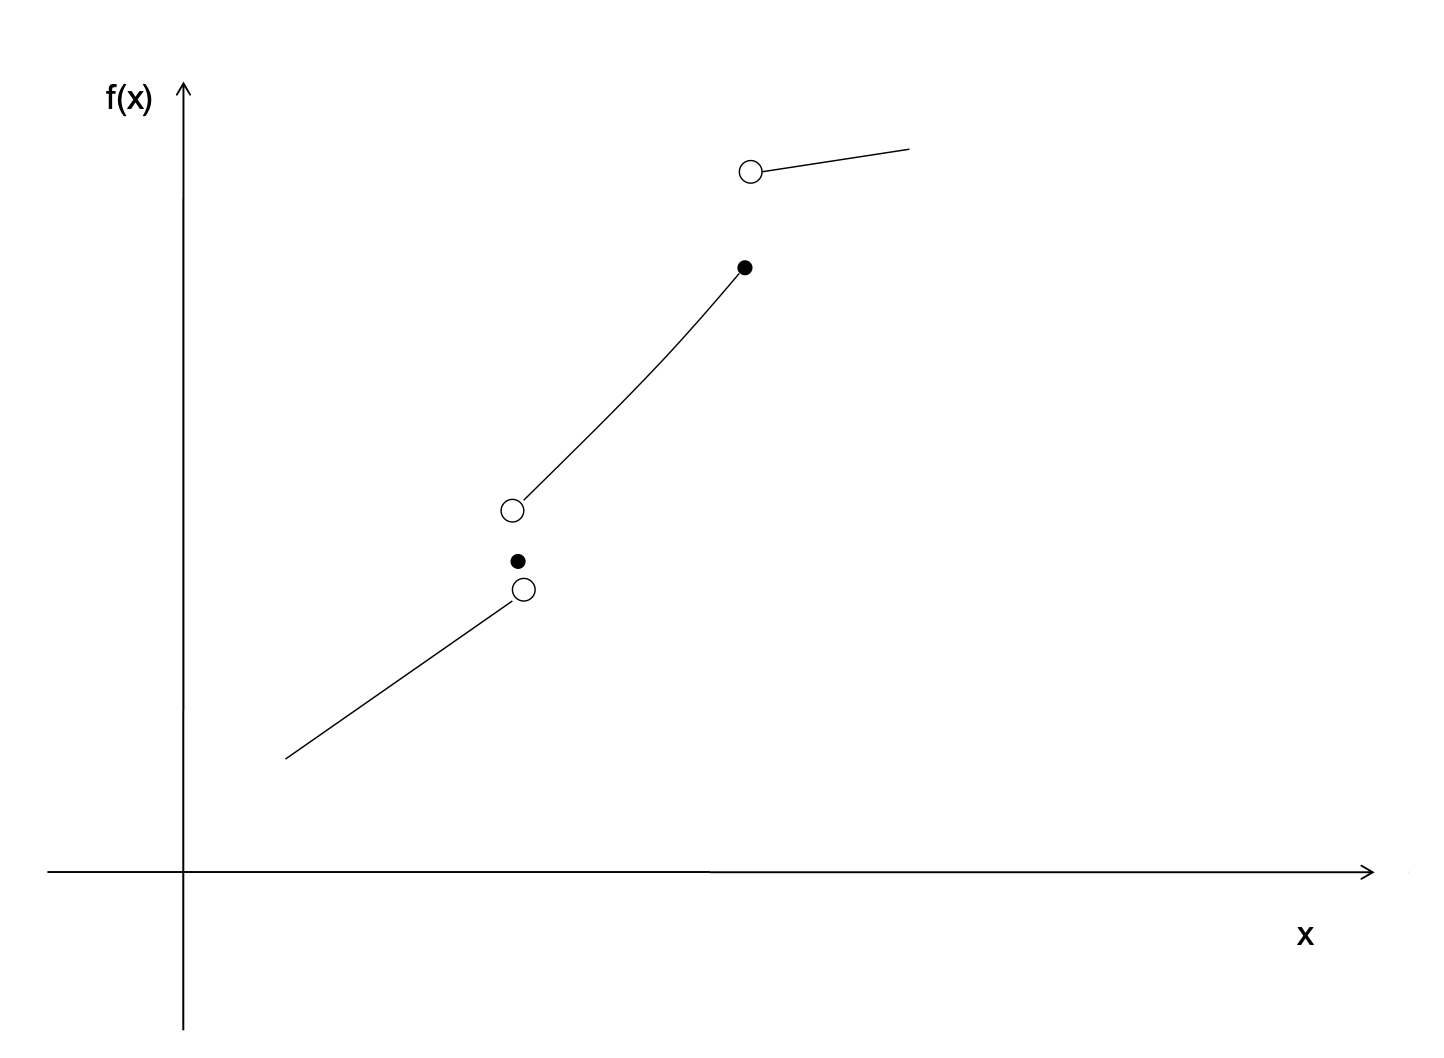
\includegraphics[scale=0.2]{SJD.png}
    \caption{A monotonic function has only simple jump discontinuities.}
    \label{}
\end{figure}\end{center}

\subsection{Theorem: Monotonically Increasing $\Rightarrow$ Set of Points are discontinuous is finite (possibly empty) or countable}
\begin{theorem}
    Let $a, b \in \mathbb{R}$ with $a < b$, and let $f : (a, b) \rightarrow \mathbb{R}$ be monotonically increasing. Then $D=\{t\in(a,b): f \textnormal{ is discontinuous at }t\}$ is finite (possibly empty) or countable.
\end{theorem}

\section{Differentiable Function \small{(@ Lec 11 of ECON 204)}}
\subsection{Definition of Differentiable in $\mathbb{R}$}
\begin{definition}
    \normalfont
    Let $f: I \rightarrow \mathbb{R}$, where $I \subseteq \mathbb{R}$ is an open interval. $f$ is \textbf{differentiable} at $x \in I$ if
    $$
    \lim _{h \rightarrow 0} \frac{f(x+h)-f(x)}{h}=a
    $$
    for some $a \in \mathbb{R}$.
\end{definition}
This is equivalent to $\exists a \in \mathbb{R}$ such that:
$$
\begin{aligned}
& \lim _{h \rightarrow 0} \frac{f(x+h)-(f(x)+a h)}{h}=0 \\
\Leftrightarrow & \forall \varepsilon>0 \exists \delta>0 \text { s.t. } 0<|h|<\delta \Rightarrow\left|\frac{f(x+h)-(f(x)+a h)}{h}\right|<\varepsilon \\
\Leftrightarrow & \forall \varepsilon>0 \exists \delta>0 \text { s.t. } 0<|h|<\delta \Rightarrow \frac{|f(x+h)-(f(x)+a h)|}{|h|}<\varepsilon \\
\Leftrightarrow & \lim _{h \rightarrow 0} \frac{|f(x+h)-(f(x)+a h)|}{|h|}=0
\end{aligned}
$$
Recall that the limit considers $h$ near zero, but not $h=0$.

\begin{proposition}
    $f$ is \textbf{differentiable} $\Rightarrow$ $f$ is \textbf{continuous}.
\end{proposition}

\subsection{General Definition of Differentiable}
\begin{definition}
    \normalfont
    If $X \subseteq \mathbb{R}^n$ is \underline{open}, $f : X \rightarrow \mathbb{R}^m$ is \textbf{differentiable} at $x \in X$ if $\exists T_x\in L(\mathbb{R}^n,\mathbb{R}^m)$ s.t. $$\lim_{h \rightarrow 0, h\in \mathbb{R}^n}\frac{|f(x+h)-(f(x)+T_x(h))|}{|h|}=0$$
    $f$ is differentiable if it is differentiable at all $x \in X$.
\end{definition}
Note that $T_x$ is uniquely determined by Equation (1). $h$ is a small, nonzero element of $\mathbb{R}^n$; $h \rightarrow 0$ from any direction, from above, below, along a spiral, etc. The definition requires that one linear operator $T_x$ works no matter how $h$ approaches zero. In this case, $f(x) + T_x(h)$ is the best linear approximation to $f(x + h)$ for small $h$.

\subsection{"$O$" and "$o$" Notations}
\begin{definition}["$O$" and "$o$"]
    \normalfont
    \begin{enumerate}
        \item $y = O(|h|^n)$ as $h \rightarrow 0$ -- read “$y$ is big-Oh of $|h|^n$” -- means $\exists K, \delta > 0$ s.t. $|h| < \delta \Rightarrow |y| \leq K|h|^n$
        \item $y = o(|h|^n)$ as $h \rightarrow 0$ -- read “$y$ is little-Oh of $|h|^n$” -- means $\lim_{h \rightarrow 0}\frac{|y|}{|h|^n}=0$
    \end{enumerate}
\end{definition}
\begin{note}
    Note that the statement $y = O(|h|^{n+1})$ as $h \rightarrow 0$ implies $y = o(|h|^n)$ as $h \rightarrow 0$.
\end{note}
In both cases, $y \rightarrow 0$ as $h \rightarrow 0$, but the \textit{rate} is different.

\begin{definition}[New Definition]
    \normalfont
    Using this notation, note that $f$ is \textbf{differentiable} at $x$ $\Leftrightarrow$
    \begin{center}
        $\exists T_x\in L(\mathbb{R}^n,\mathbb{R}^m)$ such that $f(x+h)=f(x)+T_x(h)+o(|h|)\textnormal{ as }h \rightarrow 0$
    \end{center}
\end{definition}

\subsection{Jacobian and Error Term}
\begin{definition}[Jacobian, Error Term]
    \normalfont
\begin{enumerate}[$\circ$]
    \item $d f_x$ is the linear transformation $T_x$
    \item $D f(x)$ is the matrix of $d f_x$ with respect to the standard basis. This is called the \textbf{Jacobian} or Jacobian matrix of $f$ at $x$
    \item $E_f(h)=f(x+h)-\left(f(x)+d f_x(h)\right)$ is the \textbf{error term}\\
    Using this notation, $f$ is differentiable at $x \Leftrightarrow E_f(h)=o(h)$ as $h \rightarrow 0$
\end{enumerate}
\end{definition}
Now compute $D f(x)=\left(a_{i j}\right)$. Let $\left\{e_1, \ldots, e_n\right\}$ be the standard basis of $\mathbb{R}^n$. Look in direction $e_j$ (note that $\left|\gamma e_j\right|=|\gamma|$ ).
$$
\begin{aligned}
o(\gamma)&=f\left(x+\gamma e_j\right)-\left(f(x)+T_x\left(\gamma e_j\right)\right) \\
&=f\left(x+\gamma e_j\right)-\left(f(x)+\left(\begin{array}{ccccc}
a_{11} & \cdots & a_{1 j} & \cdots & a_{1 n} \\
\vdots & \ddots & \vdots & \ddots & \vdots \\
a_{m 1} & \cdots & a_{m j} & \cdots & a_{m n}
\end{array}\right)\left(\begin{array}{c}
0 \\
\vdots \\
0 \\
\gamma \\
0 \\
\vdots \\
0
\end{array}\right)\right) \\
&=f\left(x+\gamma e_j\right)-\left(f(x)+\left(\begin{array}{c}
\gamma a_{1 j} \\
\vdots \\
\gamma a_{m j}
\end{array}\right)\right)
\end{aligned}
$$
For $i = 1, . . . , m$, let $f^i$ denote the $i^\textnormal{th}$ component of the function $f$:
\begin{equation}
    \begin{aligned}
        f^i(x+\gamma e_j)-(f^i(x)+\gamma a_{ij})&=o(\gamma)\\
        \textnormal{so, }a_{ij}&=\frac{\partial f^i}{\partial x_j}(x)
    \end{aligned}
    \nonumber
\end{equation}

\subsection{Theorem: Differentiable $\Rightarrow$ Partial Derivatives (and Jacobian) exist}
\begin{theorem}[Differentiable $\Rightarrow$ Partial Derivatives (and Jacobian) exist]
    Suppose $X \subseteq \mathbb{R}^n$ is open and $f: X \rightarrow \mathbb{R}^m$ is differentiable at $x \in X$. Then $\frac{\partial f^i}{\partial x_j}$ exists at $x$ for $1 \leq i \leq m, 1 \leq j \leq n$, and
    $$
    D f(x)=\left(\begin{array}{ccc}
    \frac{\partial f^1}{\partial x_1}(x) & \cdots & \frac{\partial f^1}{\partial x_n}(x) \\
    \vdots & \ddots & \vdots \\
    \frac{\partial f^m}{\partial x_1}(x) & \cdots & \frac{\partial f^m}{\partial x_n}(x)
    \end{array}\right)
    $$
    i.e. the Jacobian at $x$ is the matrix of partial derivatives at $x$.
\end{theorem}
\begin{note}
    If $f$ is differentiable at $x$, then all first-order partial derivatives $\frac{\partial f^i}{\partial x_j}$ exist at $x$. However, the converse is false: existence of all the first-order partial derivatives does not imply that $f$ is differentiable.
\end{note}
\begin{example}
    $f(X)=\left\{\begin{matrix}
        \frac{x_1x_2}{x_1^2+x_2^2},&X\neq (0,0)\\
        0,& X=(0,0)
    \end{matrix}\right.$
\end{example}

\subsection{Theorem: Partial Derivatives exist and Continuous $\Rightarrow$ Differentiable}
The missing piece is continuity of the partial derivatives:
\begin{theorem}[Partial Derivatives exist and Continuous $\Rightarrow$ Differentiable]
    If all the first-order partial derivatives $\frac{\partial f^i}{\partial x_j}(1 \leq i \leq m, 1 \leq j \leq$ $n)$ exist and are continuous at $x$, then $f$ is differentiable at $x$.
\end{theorem}

\subsection{Directional Derivatives}
Suppose $X \subseteq \mathbb{R}^n$ open, $f: X \rightarrow \mathbb{R}^m$ is differentiable at $x$, and $|u|=1$.
$$
\begin{aligned}
& f(x+\gamma u)-\left(f(x)+T_x(\gamma u)\right)=o(\gamma) \text { as } \gamma \rightarrow 0 \\
& \quad \Rightarrow f(x+\gamma u)-\left(f(x)+\gamma T_x(u)\right)=o(\gamma) \text { as } \gamma \rightarrow 0 \\
& \quad \Rightarrow \lim _{\gamma \rightarrow 0} \frac{f(x+\gamma u)-f(x)}{\gamma}=T_x(u)=Df(x) u
\end{aligned}
$$
i.e. the \textbf{directional derivative} in the direction $u$ (with $|u|=1$ ) is
$$
Df(x) u \in \mathbb{R}^m
$$


\subsection{Chain Rule: $d F_{x_0}= d g_{f(x_0)} \circ d f_{x_0}$ and $D F_{x_0}= D g (f(x_0)) D f (x_0)$}
\begin{theorem}[Chain Rule]
    Let $X \subseteq \mathbb{R}^n$, $Y \subseteq \mathbb{R}^m$ be open, $f : X \rightarrow Y$, $g : Y \rightarrow \mathbb{R}^p$. Let $x_0\in X$ and $F = g \circ f$. If $f$ is differentiable at $x_0$ and $g$ is differentiable at $f(x_0)$, then $F = g \circ f$ is differentiable at $x_0$ and
    \begin{equation}
        \begin{aligned}
            d F_{x_0}&= d g_{f(x_0)} \circ d f_{x_0} \textnormal{ (composition of linear transformations)}\\
            D F_{x_0}&= D g (f(x_0)) D f (x_0) \textnormal{ (matrix multiplication)}\\
        \end{aligned}
        \nonumber
    \end{equation}
\end{theorem}

\subsection{Mean Value Theorem: $\exists z\in l(x,y),\|f(y)-f(x)\|\leq \|df_z\| \|y-x\|$}
\begin{theorem}[Mean Value Theorem, Univariate Case: $\mathbb{R} \rightarrow \mathbb{R}$]
    Let $a, b \in \mathbb{R}$. Suppose $f : [a, b] \rightarrow \mathbb{R}$ is continuous on $[a, b]$ and differentiable on $(a, b)$. Then there exists $c \in (a, b)$ such that $$\frac{f(b)-f(a)}{b-a}=f'(c)$$
    that is $$f(b)-f(a)=f'(c)(b-a)$$
\end{theorem}
\begin{note}
    The Mean Value Theorem is useful for estimating bounds on functions and error terms in approximation of functions.
\end{note}

\begin{definition}[Line Segment]
    \normalfont
    $l(x,y)=\{\alpha x + (1-\alpha)y:\alpha\in[0,1]\}$ is the \textbf{line segment} from $x$ to $y$.
\end{definition}

\begin{theorem}[Mean Value Theorem, $\mathbb{R}^n \rightarrow \mathbb{R}$]
    Suppose $f : \mathbb{R}^n \rightarrow \mathbb{R}$ is differentiable on an open set $X \subseteq \mathbb{R}^n$, $x, y \in X$ and $l(x, y) \subseteq X$. Then there exists $z \in l(x, y)$ such that $$f(y)-f(x)=Df(z)(y-x)$$
\end{theorem}

\begin{theorem}[Mean Value Theorem, General Case: $\mathbb{R}^n \rightarrow \mathbb{R}^m$]
    Suppose $X \subseteq \mathbb{R}^n$ is open and $f : X \rightarrow \mathbb{R}^m$ is differentiable. If $x, y \in X$ and $l(x, y) \subseteq X$, then there exists $z \in l(x, y)$ such that
    \begin{equation}
        \begin{aligned}
            \|f(y)-f(x)\|&\leq\|df_z(y-x)\|\\
            &\leq \|df_z\| \|y-x\|
        \end{aligned}
        \nonumber
    \end{equation}
\end{theorem}


\subsection{Taylor's Theorem}
\begin{theorem}[Taylor's Theorem]
    Let $f : I \rightarrow \mathbb{R}$ be $n$-times differentiable, where $I \subseteq \mathbb{R}$ is an open interval. If $x, x + h \in I$, then
    \begin{equation}
        \begin{aligned}
            f(x+h)=f(x)+\sum_{k=1}^{n-1}\frac{f^{(k)}(x)h^k}{k!}+E_n
        \end{aligned}
        \nonumber
    \end{equation}
    where $f^{(k)}$ is the $k^\textnormal{th}$ derivative of $f$ and
    \begin{equation}
        \begin{aligned}
            E_n=\frac{f^{(n)}(x+\lambda h)h^n}{n!} \textnormal{ for some }\lambda\in(0,1)
        \end{aligned}
        \nonumber
    \end{equation}
\end{theorem}

\begin{theorem}[Taylor's Theorem in $\mathbb{R}^1$]
    Let $f : I \rightarrow \mathbb{R}$ be $n$ times differentiable, where $I \subseteq \mathbb{R}$ is an open interval and $x \in I$. Then,
    \begin{equation}
        \begin{aligned}
            f(x+h)=f(x)+\sum_{k=1}^{n}\frac{f^{(k)}(x)h^k}{k!}+o(h^n) \textnormal{ as }h \rightarrow 0
        \end{aligned}
        \nonumber
    \end{equation}
    If $f$ is $(n + 1)$ times continuously differentiable (i.e. all derivatives up to order $n + 1$ exist and are continuous), then
    \begin{equation}
        \begin{aligned}
            f(x+h)=f(x)+\sum_{k=1}^{n}\frac{f^{(k)}(x)h^k}{k!}+o(h^{n+1}) \textnormal{ as }h \rightarrow 0
        \end{aligned}
        \nonumber
    \end{equation}
\end{theorem}

\subsection{$C^k$ Function and Continuously Differentiable}
\begin{definition}[$C^k$ Function]
    \normalfont
    $f$ is $C^k$ if all partial derivatives of order less than or equal to $k$ exist and are continuous in $X$.
\end{definition}

\begin{definition}[Continuously Differentiable]
    \normalfont
    Let $X \subseteq \mathbb{R}^n$ be open. A function $f : X \rightarrow \mathbb{R}^m$ is \textbf{continuously differentiable} on $X$ if
    \begin{enumerate}
        \item $f$ is differentiable on $X$ and
        \item $df_x$ is a continuous function of $x$ from $X$ to $L(\mathbb{R}^n, \mathbb{R}^m)$, with operator norm $\|df_x\|$.
    \end{enumerate}
\end{definition}

\begin{theorem}[Continuously Differentiable $\Leftrightarrow$ $C^1$]
    Suppose $X \subseteq \mathbb{R}^n$ is open and function $f : X \rightarrow \mathbb{R}^m$ is \textbf{continuously differentiable} if and only if $f$ is $C^1$.
\end{theorem}

\subsection{Taylor's Theorem with $C^k$}
\subsubsection*{Linear Terms}
\begin{theorem}
    Suppose $X \subseteq \mathbb{R}^n$ is open and $x \in X$. If $f: X \rightarrow \mathbb{R}^m$ is differentiable, then
    $$
    f(x+h)=f(x)+D f(x) h+o(h) \text { as } h \rightarrow 0
    $$
\end{theorem}
The previous theorem is essentially a restatement of the definition of differentiability.

\begin{theorem}
    Suppose $X \subseteq \mathbb{R}^n$ is open and $x \in X$. If $f: X \rightarrow \mathbb{R}^m$ is $C^2$, then
    $$
    f(x+h)=f(x)+D f(x) h+O\left(|h|^2\right) \text { as } h \rightarrow 0
    $$
\end{theorem}

\subsubsection*{Quadratic Terms}
We treat each component of the function separately, so consider $f: X \rightarrow \mathbb{R}, X \subseteq \mathbb{R}^n$ an open set. Let
$$
\begin{aligned}
D^2 f(x) & =\left(\begin{array}{cccc}
\frac{\partial^2 f}{\partial x_1^2}(x) & \frac{\partial^2 f}{\partial x_2 \partial x_1}(x) & \cdots & \frac{\partial^2 f}{\partial x_n \partial x_1}(x) \\
\frac{\partial^2 f}{\partial x_1 \partial x_2}(x) & \frac{\partial^2 f}{\partial x_2^2}(x) & \cdots & \frac{\partial^2 f}{\partial x_n \partial x_2}(x) \\
\vdots & \vdots & \ddots & \vdots \\
\frac{\partial^2 f}{\partial x_1 \partial x_n}(x) & \cdots & \cdots & \frac{\partial^2 f}{\partial x_n^2}(x)
\end{array}\right) \\
f \in C^2 & \Rightarrow \frac{\partial^2 f}{\partial x_i \partial x_j}(x)=\frac{\partial^2 f}{\partial x_j \partial x_i}(x) \\
& \Rightarrow D^2 f(x) \text { is symmetric } \\
& \Rightarrow D^2 f(x) \text { has an orthonormal basis of eigenvectors and thus can be diagonalized}
\end{aligned}
$$

\begin{theorem}[Stronger Version of Taylor's Theorem]
    Suppose $X \subseteq \mathbb{R}^n$ is open and $x \in X$. If $f: X \rightarrow \mathbb{R}$ is $C^2$, then
    $$
    f(x+h)=f(x)+D f(x) h +\frac{1}{2}h^T(D^2f(x))h+O\left(|h|^2\right) \text { as } h \rightarrow 0
    $$
    If $f\in C^3$,
    $$
    f(x+h)=f(x)+D f(x) h +\frac{1}{2}h^T(D^2f(x))h+O\left(|h|^3\right) \text { as } h \rightarrow 0
    $$
\end{theorem}

\begin{definition}
    \normalfont
    We say $f$ has a \textbf{saddle} at $x$ if $D f(x)=0$ but $f$ has neither a local maximum nor a local minimum at $x$.
\end{definition}

\begin{corollary}
    Suppose $X \subseteq \mathbb{R}^n$ is open and $x \in X$. If $f: X \rightarrow \mathbb{R}$ is $C^2$, then there is an orthonormal basis $\left\{v_1, \ldots, v_n\right\}$ and corresponding eigenvalues $\lambda_1, \ldots, \lambda_n \in \mathbb{R}$ of $D^2 f(x)$ such that
    $$
    \begin{aligned}
    f(x+h) & =f\left(x+\gamma_1 v_1+\cdots+\gamma_n v_n\right) \\
    & =f(x)+\sum_{i=1}^n\left(D f(x) v_i\right) \gamma_i+\frac{1}{2} \sum_{i=1}^n \lambda_i \gamma_i^2+o\left(|\gamma|^2\right)
    \end{aligned}
    $$
    where $\gamma_i=h \cdot v_i$.
    \begin{enumerate}[1.]
        \item If $f \in C^3$, we may strengthen $o\left(|\gamma|^2\right)$ to $O\left(|\gamma|^3\right)$.
        \item If $f$ has a local maximum or local minimum at $x$, then
        $$
        D f(x)=0
        $$
        \item If $D f(x)=0$, then
        $$
        \begin{array}{rl}
        \lambda_1, \ldots, \lambda_n>0 & \Rightarrow f \text { has a local minimum at } x \\
        \lambda_1, \ldots, \lambda_n<0 & \Rightarrow f \text { has a local maximum at } x \\
        \lambda_i<0 \text { for some } i, \lambda_j>0 \text { for some } j & \Rightarrow f \text { has a saddle at } x \\
        \lambda_1, \ldots, \lambda_n \geq 0, \lambda_i>0 \text { for some } i &\Rightarrow f \text { has a local minimum or a saddle at } x \\
        \lambda_1, \ldots, \lambda_n \leq 0, \lambda_i<0 \text { for some } i &\Rightarrow f \text { has a local maximum or a saddle at } x \\
        \lambda_1=\cdots=\lambda_n=0 &\quad \text{ gives no information. }
        \end{array}
        $$
    \end{enumerate}
\end{corollary}


\chapter{Tools for Comparative Statics}
Consider the function $f:(0,2\pi) \times \mathbb{R} \rightarrow \mathbb{R}$ s.t. $$f(x,a)=\sin x+a$$
Let $X=(0,2\pi)$ and let $f_a(x) = f(x, a) = \sin x + a$ denote the perturbed function for fixed $a$.



\section{Regular and Critical Points and Values}
\subsection{Rank of Derivatives $\textnormal{Rank} df_x=\textnormal{Rank} Df(x)$}
Suppose $X \subseteq \mathbb{R}^n$ is open. Suppose $f : X \rightarrow \mathbb{R}^m$ is differentiable at $x \in X$, and let $W = \{e_1, . . . , e_n\}$ denote the standard basis of $\mathbb{R}^n$. Then $df_x \in L(\mathbb{R}^n, \mathbb{R}^m)$, and
\begin{equation}
    \begin{aligned}
        \textnormal{Rank} df_x &= \dim \textnormal{Im}(df_x)\\
        &= \dim \textnormal{span}\{df_x(e_1), . . . , df_x(e_n)\}\\
        &= \dim \textnormal{span}\{Df(x)e_1, . . . , Df(x)e_n\}\\
        &= \dim \textnormal{span}\{\textnormal{column 1 of }Df(x), . . . , \textnormal{column n of }Df(x)\}\\
        &=\textnormal{Rank} Df(x)
    \end{aligned}
    \nonumber
\end{equation}
Thus,
$$\textnormal{Rank} df_x\leq\min\{m,n\}$$
$df_x$ has \textbf{full rank} if $\textnormal{Rank} df_x=\min\{m,n\}$, that is, is $df_x$ has the maximum possible rank.

\subsection{Regular and Critical Points and Values}
\begin{definition}[Regular and Critical Points and Values]
    \normalfont
    Suppose $X \subseteq \mathbb{R}^n$ is open. Suppose $f : X \rightarrow \mathbb{R}^m$ is differentiable at $x \in X$.
    \begin{enumerate}
        \item $x$ is a \textbf{regular point} of $f$ if $\textnormal{Rank} df_x=\min\{m,n\}$.
        \item $x$ is a \textbf{critical point} of $f$ if $\textnormal{Rank} df_x<\min\{m,n\}$.
        \item $y$ is a \textbf{critical value} of $f$ if  there exists $x \in f^{-1}(y)$ such that $x$ is a critical point of $f$.
        \item $y$ is a \textbf{regular value} of $f$ if $y$ is not a critical value of $f$.
    \end{enumerate}
\end{definition}
\begin{note}
    Notice that if $y \notin f(X)$, so $f^{-1}(y) = \emptyset$, then $y$ is automatically a regular value of $f$.
\end{note}

\begin{example}
    Suppose $f(x,y)=(\sin x,\cos y)$, $Df(x,y)=\begin{bmatrix}
        \cos x&	0\\
        0&	-\sin y
    \end{bmatrix}$. Critical point: $\{(\frac{k\pi}{2}, \mathbb{R}): k\in 2\mathbb{Z}+1\}\cup\{(\mathbb{R},k\pi): k\in \mathbb{Z}\}$; Critical values: $\{(x,y): x=1\textnormal{ or }x=-1 \textnormal{ or }y=1\textnormal{ or }y=-1\}$
\end{example}


\section{Inverse and Implicit Function Theorem}
\subsection{Inverse Function Theorem}
Using Taylor's theorem to approximate
\begin{equation}
    \begin{aligned}
        f(x)=f(x_0)+Df(x_0)(x-x_0)+o(x-x_0)
    \end{aligned}
    \nonumber
\end{equation}
The requirement of "regular point" is necessary for the $Df(x_0)$ being invertible.
\begin{theorem}[Inverse Function Theorem]
    Suppose $X \subseteq \mathbb{R}^n$ is open. Suppose $f : X \rightarrow \mathbb{R}^n$ is $C^1$ on $X$, and $x_0\in X$. If $\det Df(x_0)\neq 0$ (i.e., $x_0$ is a regular point of $f$), then there are open neighborhoods $U$ of $x_0$ and $V$ of $f(x_0)$ s.t.
    \begin{equation}
        \begin{aligned}
            &f:U \rightarrow V \textnormal{ is bijective (on-to-on and onto)}\\
            &\exists\ f^{-1}:V \rightarrow U \textnormal{ is }C^1\\
            &Df^{-1}(f(x_0))=[Df(x_0)]^{-1}\\
            &\textnormal{(In $\mathbb{R}$, $(f^{-1})'(f(x_0))=(f'(x_0))^{-1}$)}
        \end{aligned}
        \nonumber
    \end{equation}
    If in addition $f \in C^k$, then $f^{-1} \in C^k$.
\end{theorem}

\subsection{Implicit Function Theorem}
Using Taylor's theorem to approximate
\begin{equation}
    \begin{aligned}
        f(x,a)=f(x_0,a_0)+Df(x_0,a_0)(x-x_0)+Df(x_0,a_0)(a-a_0)+\textnormal{remainder}
    \end{aligned}
    \nonumber
\end{equation}
The requirement of "regular point" is necessary for the $Df(x_0,a_0)$ being invertible.

We want to know how the function $x^*(a)$ changes with keeping $f(x^*,a)=0$.
\begin{theorem}[Implicit Function Theorem]
    Suppose $X \subseteq \mathbb{R}^n$ and $A \subseteq \mathbb{R}^p$ are open and $f : X \times A \rightarrow \mathbb{R}^n$ is $C^1$. Suppose $f(x_0, a_0) = 0$ and $\det(D_x f(x_0, a_0)) \neq 0$, i.e. $x_0$ is a regular point of $f(\cdot, a_0)$. Then there are open neighborhoods $U$ of $x_0$ ($U \subseteq X$) and $W$ of $a_0$ such that
    $$\forall a\in W,\ \exists ! x\in U \textnormal{ s.t. }f(x,a)=0$$
    For each $a \in W$ let $g(a)$ be that unique $x$. Then $g : W \rightarrow U$ is $C^1$ and $$Dg(a_0)=-[D_x f(x_0, a_0)]^{-1}[D_a f(x_0, a_0)]$$
    If in addition $f \in C^k$, then $g \in C^k$.
\end{theorem}
\subsection{Prove Implicit Function Theorem Given Inverse Function Theorem}
\begin{proof}
    \begin{enumerate}
        \item Firstly, we prove "$g$ is differentiable":
        The "change of $a$" incurs the value change:
        \begin{equation}
            \begin{aligned}
                f(x_0,a_0+h)&=f(x_0,a_0)+D_af(x_0,a_0)h+o(h)\\
                &=D_af(x_0,a_0)h+o(h)\\
            \end{aligned}
            \nonumber
        \end{equation}
        Find a $\Delta x$ such that the new $x$ can let the value go back to $0$, i.e., $f(x_0+\Delta x,a_0+h)=0$. That is,
        \begin{equation}
            \begin{aligned}
                g(a_0+h)=x_0+\Delta x
            \end{aligned}
            \nonumber
        \end{equation}
        To prove "$g$ is differentiable", we want to prove "$\exists T\in L(A,X)$ s.t. $\Delta x=T(h)+o(h)$"
        \begin{equation}
            \begin{aligned}
                0&=f(x_0+\Delta x,a_0+h)\\
                &=f(x_0,a_0)+D_xf(x_0,a_0+h)\Delta x+ D_a f(x_0,a_0)h+o(\Delta x)+o(h)\\
                &=D_xf(x_0,a_0+h)\Delta x+ D_a f(x_0,a_0)h+o(\Delta x)+o(h)\\
                D_x f(x_0,a_0+h)\Delta x&=-D_a f(x_0,a_0)h+o(\Delta x)+o(h)
            \end{aligned}
            \nonumber
        \end{equation}
        Because $f$ is $C^1$ and the determinant is a continuous function of the entries of the matrix, $\det D_xf(x_0, a_0 + h) \neq 0$ for $h$ sufficiently small, so
        \begin{equation}
            \begin{aligned}
                \Delta x&= -[D_x f(x_0,a_0+h)]^{-1}D_a f(x_0,a_0)h+o(\Delta x)+o(h)\\
                \textnormal{Since $f\in C^1$, }\Delta x&= -[D_x f(x_0,a_0)+o(1)]^{-1}D_a f(x_0,a_0)h+o(\Delta x)+o(h)\\
                \textnormal{Since $f\in C^1$, }\Delta x&= -[D_x f(x_0,a_0)]^{-1}D_a f(x_0,a_0)h+o(\Delta x)+o(h)
            \end{aligned}
            \nonumber
        \end{equation}
        Hence, "$g$ is differentiable" is proved and the derivative of $g$ is $Dg(a_0)=-[D_x f(x_0,a_0)]^{-1}[D_a f(x_0,a_0)]$.
        \item Secondly, given the "$g$ is differentiable", we can also compute the derivative by
        \begin{equation}
            \begin{aligned}
                Df(g(a),a)(a_0)&=0\\
                D_xf(x_0,a_0)Dg(a_0)+D_af(x_0,a_0)&=0\\
                Dg(a_0)&=-[D_x f(x_0,a_0)]^{-1}D_a f(x_0,a_0)
            \end{aligned}
            \nonumber
        \end{equation}
    \end{enumerate}
\end{proof}







\begin{example}
    $f: \mathbb{R}^3 \rightarrow \mathbb{R}^2$, $f((3,-1,2))=(0,0)$, $Df(3,-1,2)=\begin{bmatrix}
        1&2&1\\
        1&-1&1
    \end{bmatrix}$. Then,
    let $(x_0,a_0)=(3,-1,2)$, where $x_0=3$ and $a_0=(-1,2)$. Or, we can let $(x_0,a_0)=(3,-1,2)$, where $x_0=(3,-1)$ and $a_0=2$.
\end{example}

\subsection{Prove Inverse Function Theorem Given Implicit Function Theorem}
\begin{proof}[Prove Inverse Function Theorem Given Implicit Function Theorem]
    Define $F:X\times \mathbb{R}^n$ s.t. $F(x,y)=y-f(x)$. Let $y_0=f(x_0)$.
    \begin{equation}
        \begin{aligned}
            D_x F(x,y)=-Df(x),\ D_y F(x,y)=I_{n\times n}
        \end{aligned}
        \nonumber
    \end{equation}
    According to the implicit function theorem, there are open sets $U \subseteq X$ and $V \subseteq \mathbb{R}^n$ such that $x_0 \in U$, $y_0 \in V$ and a function $g : V \rightarrow U$ differentiable at $y_0$ such that $F(g(y), y) = 0$ for all $y \in V$. So, $0=F(g(y),y)=y-f(g(y))$, we have $f(g(y))=y$, that is $g=f^{-1}$.
    $f: U \rightarrow V$ is bijective because it has inverse $g : V \rightarrow U$.

    By the implicit function theorem, $g(y)$ is differentiable and
    \begin{equation}
        \begin{aligned}
            Df^{-1}(y_0)=Dg(y_0)=-[D_x F(x_0,y_0)]^{-1}[D_y F(x_0,y_0)]=[Df(x_0)]^{-1}
        \end{aligned}
        \nonumber
    \end{equation}
    where $y_0=f(x_0)$.
    
    By the implicit function theorem, the $g=f^{-1}$ is $C^k$ if $f$ is $C^k$.

    All in all, the inverse function theorem is proved.
\end{proof}

\subsection{Example: Using Implicit Function Theorem in Comparative Statics}
\begin{example}
    Let us consider a firm that produces a good $y$; it uses two inputs $x_1$ and $x_2$. The firm sells the output and acquires the inputs in competitive markets: The market price of $y$ is $p$, and the cost of each unit of $x_1$ and $x_2$ are $w_1$ and $w_2$ respectively. Its technology is given by $f : \mathbb{R}^2_+ \rightarrow \mathbb{R}_+$, where $f (x_1, x_2) = x_1^ax_2^b$, $a + b < 1$. Its profits take the form
    \begin{equation}
        \begin{aligned}
            \pi(x_1,x_2; p, w_1,w_2)=p x_1^ax_2^b-w_1x_1-w_2x_2
        \end{aligned}
        \nonumber
    \end{equation}
    The firm selects $x_1$ and $x_2$ in order to maximize profits. \textbf{We aim to know how its choice of $x_1$ and $x_2$ is affected by a change in $w_1$}.

    Assuming an interior solution, the first-order conditions of this optimization problem are
    \begin{equation}
        \begin{aligned}
            \frac{\partial \pi}{\partial x_1}(x_1^*,x_2^*;p,w_1,w_2)=pa(x_1^*)^{a-1}(x_2^*)^b-w_1=0\\
            \frac{\partial \pi}{\partial x_2}(x_1^*,x_2^*;p,w_1,w_2)=pb(x_1^*)^{a}(x_2^*)^{b-1}-w_2=0
        \end{aligned}
        \nonumber
    \end{equation}
    for some $(x_1, x_2) = (x_1^*,x_2^*)$.

    Let us define
    \begin{equation}
        \begin{aligned}
            F(x_1^*,x_2^*;p,w_1,w_2)=
            \begin{bmatrix}
                pa(x_1^*)^{a-1}(x_2^*)^b-w_1\\
                pb(x_1^*)^{a}(x_2^*)^{b-1}-w_1
            \end{bmatrix}
        \end{aligned}
        \nonumber
    \end{equation}
    Jacobian matrices are
    \begin{equation}
        \begin{aligned}
            D_{(x_1,x_2)}F(x_1^*,x_2^*;p,w_1,w_2)=\begin{bmatrix}
                pa(a-1)(x_1^*)^{a-2}(x_2^*)^b&pab(x_1^*)^{a-1}(x_2^*)^{b-1}\\
                pab(x_1^*)^{a-1}(x_2^*)^{b-1}&pb(b-1)(x_1^*)^{a}(x_2^*)^{b-2}
            \end{bmatrix}
        \end{aligned}
        \nonumber
    \end{equation}
    \begin{equation}
        \begin{aligned}
            D_{w_1}F(x_1^*,x_2^*;p,w_1,w_2)
            &=
            \begin{bmatrix}
                -1\\
                0
            \end{bmatrix}
        \end{aligned}
        \nonumber
    \end{equation}
    By the implicit function theorem, we can get
    \begin{equation}
        \begin{aligned}
            \begin{bmatrix}
                \frac{\partial x_1^*}{\partial w_1}\\
                \frac{\partial x_2^*}{\partial w_1}
            \end{bmatrix}&=-[D_{(x_1,x_2)}F(x_1^*,x_2^*;p,w_1,w_2)]^{-1}[D_{w_1}F(x_1^*,x_2^*;p,w_1,w_2)]\\
            &=[D_{(x_1,x_2)}F(x_1^*,x_2^*;p,w_1,w_2)]^{-1}\begin{bmatrix}
                1\\
                0
            \end{bmatrix}
        \end{aligned}
        \nonumber
    \end{equation}
\end{example}

\subsection{Corollary: $a \rightarrow \{x\in X: f(x,a)=0\}$ is lhc}
\begin{corollary}
    Suppose $X \subseteq \mathbb{R}^n$ and $A \subseteq \mathbb{R}^p$ are open and $f : X \times A \rightarrow \mathbb{R}^n$ is $C^1$. If $0$ is a regular value of $f(\cdot, a_0)$, then the correspondence $$a \rightarrow \{x\in X: f(x,a)=0\}$$
    is \textbf{lower hemicontinuous} at $a_0$.
\end{corollary}


\section{Transversality and Genericity}
\subsection{Lebesgue Measure Zero}
\begin{definition}[Lebesgue Measure Zero]
    \normalfont
    Suppose $A \subseteq \mathbb{R}^n$. $A$ has \textbf{Lebesgue measure zero} if for every $\varepsilon > 0$ there is a countable collection of rectangles $I_1, I_2, . . .$ such that
    \begin{equation}
        \begin{aligned}
            \sum_{k=1}^\infty\textnormal{Vol}(I_k)<\varepsilon \textnormal{ and }A\subseteq \cup_{k=1}^\infty I_k
        \end{aligned}
        \nonumber
    \end{equation}
    Here by a rectangle we mean $I_k = \times^n_{j=1}(a^k_j , b^k_j)=\{x\in \mathbb{R}^n: x_j\in (a^k_j , b^k_j), \forall j\}$ for some $a^k_j < b^k_j \in \mathbb{R}$, and
    \begin{equation}
        \begin{aligned}
            \textnormal{Vol}(I_k)=\prod_{j=1}^n|b^k_j-a^k_j|
        \end{aligned}
        \nonumber
    \end{equation}
\end{definition}

\begin{example}
    \begin{enumerate}
        \item “Lower-dimensional” sets have Lebesgue measure zero. For example, $A=\{x\in\mathbb{R}^2:x_2=0\}$
        \item Any \textbf{finite} set has Lebesgue measure zero in $\mathbb{R}^n$.
        \item \textbf{Finite Union} of sets that have Lebesgue measure zero has Lebesgue measure zero: If $A_n$ has Lebesgue measure zero $\forall n$ then $\cup_{n\in N}A_n$ has Lebesgue measure zero.
        \item Every \textbf{countable} set (e.g. $\mathbb{Q}$) has Lebesgue measure zero.
        \item No open set in $\mathbb{R}^n$ has Lebesgue measure zero.
    \end{enumerate}
\end{example}


\subsection{Sard's Theorem}
\begin{theorem}[Sard's Theorem]
    Let $X \subseteq \mathbb{R}^n$ be open, and $f : X \rightarrow \mathbb{R}^m$ be $C^r$ with $r \geq 1 + max\{0, n - m\}$. Then the set of all critical values of $f$ has Lebesgue measure zero.
\end{theorem}

\subsection{Transversality Theorem}
\begin{theorem}[Transversality Theorem]
    Let $X \subseteq \mathbb{R}^n$ and $A \subseteq \mathbb{R}^p$ be open, and $f : X \times A \rightarrow \mathbb{R}^m$ be $C^r$ with $r \geq 1 + max\{0, n - m\}$. Suppose that $0$ is a regular value of $f$ (that is all $(x,a)$ such that $f(x,a)=0$ are regular points). Then,
    \begin{enumerate}
        \item $\exists A_0 \subseteq A$ such that $A \backslash A_0$ has Lebesgue measure zero.
        \item $\forall a \in A_0$, $0$ is a regular value of $f_a = f(\cdot, a)$.
    \end{enumerate}
\end{theorem}
\begin{example}
    $f: \mathbb{R}^4 \rightarrow \mathbb{R}^3$ s.t. $f(x,y,z,w)=(g(x)+y,z^3+1,w+x+y^2)$
\end{example}


\chapter{Fixed Point Theorem}

\section{Contraction Mapping Theorem \small{(@ Lec 05 of ECON 204)}}
\subsection{Contraction of modulus $\beta$: $d(T(x), T(y)) \leq \beta d(x, y), \forall x,y\in X$}
\begin{definition}
    \normalfont
    Let $(X, d)$ be a \underline{nonempty complete} metric space. An operator is a function $T : X \rightarrow X$. An operator $T$ is a \textbf{contraction of modulus $\beta$} if $\beta < 1$ and $$d(T(x), T(y)) \leq \beta d(x, y), \forall x,y\in X$$
\end{definition}
A contraction shrinks distances by a \textit{uniform} factor $\beta < 1$.

\subsection{Theorem: Contraction $\Rightarrow$ Uniformly Continuous}
\begin{theorem}[Contraction $\Rightarrow$ Uniformly Continuous]
    Every contraction is uniformly continuous.
\end{theorem}
\begin{proof}
    Let $\delta=\frac{\varepsilon}{\beta}$.
\end{proof}

\subsection{Theorem: Blackwell's Sufficient Conditions for Contraction}
Let $X$ be a set, and let $B(X)$ be the set of all bounded functions from $X$ to $\mathbb{R}$. Then $(B(X), \|\cdot\|_\infty)$ is a normed vector space.

(Notice that below we use shorthand notation that identifies a constant function with its constant value in $\mathbb{R}$, that is, we write interchangeably $a \in \mathbb{R}$ and $a : X \rightarrow \mathbb{R}$ to denote the function such that $a(x) = a, \forall x \in X$.)

\begin{theorem}[Blackwell's Sufficient Conditions]
    Consider $B(X)$ with the sup norm $\|\cdot\|_\infty$. Let $T : B(X) \rightarrow B(X)$ be an operator satisfying
    \begin{enumerate}
        \item (monotonicity) $f(x) \leq g(x), \forall x\in X \Rightarrow (T f)(x) \leq (T g)(x), \forall x \in X$
        \item (discounting) $\exists \beta \in (0, 1)$ such that for every $a \geq 0$ and $x \in X$, $$(T (f + a)) (x) \leq (T f)(x) + \beta a$$
    \end{enumerate}
    Then $T$ is a contraction with modulus $\beta$.
\end{theorem}
\begin{proof}
    Fix $f, g \in B(X)$. By the definition of the sup norm,
    $$
    f(x) \leq g(x)+\|f-g\|_{\infty} \forall x \in X
    $$
    Then
    $$
    (T f)(x) \leq\left(T\left(g+\|f-g\|_{\infty}\right)\right)(x) \leq(T g)(x)+\beta\|f-g\|_{\infty} \quad \forall x \in X
    $$
    where the first inequality above follows from monotonicity, and the second from discounting. Thus
    $$
    (T f)(x)-(T g)(x) \leq \beta\|f-g\|_{\infty} \quad \forall x \in X
    $$
    Reversing the roles of $f$ and $g$ above gives
    $$
    (T g)(x)-(T f)(x) \leq \beta\|f-g\|_{\infty} \quad \forall x \in X
    $$
    Thus
    $$
    \|T(f)-T(g)\|_{\infty} \leq \beta\|f-g\|_{\infty}
    $$
    Thus $T$ is a contraction with modulus $\beta$
\end{proof}


\section{Fixed Point Theorem \small{(@ Lec 05 of ECON 204)}}
\subsection{Fixed Point}
\begin{definition}[Fixed Point]
    \normalfont
    A \textbf{fixed point} of an operator $T$ is element $x^*\in X$ such that $T(x^*)=x^*$.
\end{definition}

\begin{definition}[Fixed Point of Function]
    \normalfont
    Let $X$ be a nonempty set and $f : X \rightarrow X$. A point $x^* \in X$ is a \textbf{fixed point} of $f$ if $f(x^*) = x^*$.
\end{definition}

\begin{example}
    Let $X=\mathbb{R}$ and $f: \mathbb{R} \rightarrow \mathbb{R}$
    \begin{enumerate}
        \item $f(x)=2x$ has fixed point: $x=0$.
        \item $f(x)=x$ has fixed points: $x\in \mathbb{R}$.
        \item $f(x)=x+1$ doesn't have fixed points.
    \end{enumerate}
\end{example}

\subsection{Contraction Mapping Theorem: Existence and Uniqueness of Fixed Point}
\begin{theorem}[Contraction Mapping Theorem]
    Let $(X, d)$ be a nonempty complete metric space and $T : X \rightarrow X$ a contraction with modulus $\beta < 1$. Then
    \begin{enumerate}
        \item $T$ has a unique fixed point $x^*$.
        \item For every $x_0 \in X$, the sequence defined by
        \begin{equation}
            \begin{aligned}
                x_1&=T(x_0)\\
                x_2&=T(x_1)=T(T(x_0))=T^2(x_0)\\
                &\vdots\\
                x_{n+1}&=T(x_n)=T^{n+1}(x_0)
            \end{aligned}
            \nonumber
        \end{equation}
        converges to $x^*$.
    \end{enumerate}
\end{theorem}
Note that the theorem asserts both the \textbf{existence} and \textbf{uniqueness} of the fixed point, as well as giving an \textbf{algorithm} to find the fixed point of a contraction.
\begin{proof}
    Define the sequence $\{x_n\}$ as above. Then,
    \begin{equation}
        \begin{aligned}
            d(x_{n+1},x_n)&=d(T(x_n),T(x_{n-1}))\\
            &\leq \beta d(x_n,x_{n-1})\\
            &\leq \beta^n d(x_1,x_0)
        \end{aligned}
        \nonumber
    \end{equation}
    Then for any $n>m$,
    \begin{equation}
        \begin{aligned}
            d(x_n,x_m)&\leq d(x_1, x_0) \sum_{i=m}^{n-1}\beta^i\\
            &<d(x_1, x_0) \sum_{i=m}^{\infty}\beta^i\\
            &=\frac{\beta^m}{1-\beta}d(x_1, x_0) \rightarrow 0 \textnormal{ as }m \rightarrow \infty
        \end{aligned}
        \nonumber
    \end{equation}
    Fixed $\varepsilon>0$, we can choose $N(\varepsilon)$ such that $\forall n,m>N(\varepsilon)$, $$d(x_n,x_m)<\frac{\beta^m}{1-\beta}d(x_1, x_0) <\varepsilon$$
    Therefore, $\{x_n\}$ is Cauchy. Since $(X, d)$ is complete, $x_n \rightarrow x^*$ for some $x^*\in X$.

    Next we show that $x^*$ is a fixed point of $T$.
    $$
    \begin{aligned}
    T\left(x^*\right) & =T\left(\lim _{n \rightarrow \infty} x_n\right) \\
    & =\lim _{n \rightarrow \infty} T\left(x_n\right) \text { since } T \text { is continuous } \\
    & =\lim _{n \rightarrow \infty} x_{n+1} \\
    & =x^*
    \end{aligned}
    $$
    so $x^*$ is a fixed point of $T$.
    
    Finally, we show that there is at most one fixed point. Suppose $x^*$ and $y^*$ are both fixed points of $T$, so $T\left(x^*\right)=x^*$ and $T\left(y^*\right)=y^*$. Then
    $$
    \begin{aligned}
    d\left(x^*, y^*\right) & =d\left(T\left(x^*\right), T\left(y^*\right)\right) \\
    & \leq \beta d\left(x^*, y^*\right) \\
    \Rightarrow(1-\beta) d\left(x^*, y^*\right) & \leq 0 \\
    \Rightarrow d\left(x^*, y^*\right) & \leq 0
    \end{aligned}
    $$
    So $d\left(x^*, y^*\right)=0$, which implies $x^*=y^*$.
\end{proof}



\subsection{Theorem: Fixed Point's Continuous Dependence on Parameters}
\begin{theorem}[Continuous Dependence on Parameters]
    Let $(X, d)$ and $(\Omega, \rho)$ be two metric spaces and $T : X \times \Omega \rightarrow X$. For each parameter $\omega \in \Omega$ let $T_\omega : X \rightarrow X$ be defined by $T_\omega(x)=T(x,\omega)$.

    Suppose (1). $(X, d)$ is complete, (2). $T$ is continuous in $\omega$ (that is $T(x, \cdot) : \Omega \rightarrow X$ is continuous for each $x \in X$), and (3). $\exists \beta < 1$ such that $T_\omega$ is a contraction of modulus $\beta$ $\forall \omega \in \Omega$.
    
    Then the fixed point function (about parameter $\omega$) $x^*: \Omega \rightarrow X$ defined by $x^*(\omega)=T_\omega(x^*(\omega))$ is continuous.
\end{theorem}

\section{Brouwer's Fixed Point Theorem \small{(@ Lec 13 of ECON 204)}}
\subsection{Simple One: One-dimension}
\begin{theorem}
    Let $X = [a, b]$ for $a, b \in \mathbb{R}$ with $a < b$ and let $f : X \rightarrow X$ be continuous. Then $f$ has a fixed point.
\end{theorem}
\begin{proof}
    Easily proved by Intermediate Value Theorem.
\end{proof}

\subsection{Brouwer's Fixed Point Theorem}
\begin{theorem}[Brouwer's Fixed Point Theorem]
    Let $X \subseteq \mathbb{R}^n$ be nonempty, \textbf{compact}, and \textbf{convex}, and let $f : X \rightarrow X$ be continuous. Then $f$ has a fixed point.
\end{theorem}
\begin{proof}
    \normalfont
    Consider the case when the set $X$ is the unit ball in $\mathbb{R}^n$.

    Using a fact that "Let $B$ be the unit ball in $\mathbb{R}^n$. Then there is no continuous function $h : B \rightarrow \partial B$ such that $h(x_0) = x_0$ for every $x_0 \in \partial B$", which is intuitive but hard to prove. (See \textit{J. Franklin, Methods of Mathematical Economics}, for an elementary (but long) proof.)

    Then prove by contradiction: suppose $f$ has no fixed points in $B$. That is, $\forall x\in B$, $x\neq f(x)$. Since x and its image $f(x)$ are distinct points in $B$ for every $x$, we can carry out the following construction. For each $x \in B$, construct the line segment originating at $f(x)$ and going through $x$. Let $g(x)$ denote the intersection of this line segment with $\partial B$. This construction gives a continuous function $g : B \rightarrow \partial B$. Furthermore, notice that if $x_0 \in \partial B$, then $x_0 = g(x_0)$. Then, $g$ gives $g(x)=x,\forall x\in \partial B$. Since there are no such functions by the fact above, we have a contradiction.
\end{proof}




\chapter{Correspondence: $\Psi : X \rightarrow 2^Y$ \small{(@ Lec 07 of ECON 204)}}
\begin{definition}[Correspondence]
    \normalfont
    A \textbf{correspondence} $\Psi : X \rightarrow 2^Y$ from $X$ to $Y$ is a function from $X$ to $2^Y$, that is, $\Psi(x) \subseteq Y$ for every $x \in X$. ($2^Y$ is the set of all subsets of $Y$)
\end{definition}
\begin{example}
Let $u : \mathbb{R}_+^n \rightarrow \mathbb{R}$ be a continuous utility function, $y > 0$ and $p \in \mathbb{R}_{++}^n$, that is, $p_i > 0$ for each $i$. Define $\Psi : \mathbb{R}_{++}^n \times \mathbb{R}_{++} \rightarrow 2^{\mathbb{R}_{+}^n}$ by
\begin{equation}
    \begin{aligned}
        \Psi(p,y)=&\argmax u(x)\\
        \textnormal{s.t. }&x\geq 0\\
        &p\cdot x\leq y
    \end{aligned}
    \nonumber
\end{equation}
$\Psi$ is the demand correspondence associated with the utility function $u$; typically $\Psi(p, y)$ is multi-valued.
\end{example}

\section{Continuity of Correspondences}
\subsection{Upper/Lower Hemicontinuous}
Let $X\subseteq \mathbb{E}^n$, $Y\subseteq \mathbb{E}^m$, and $\Psi: X \rightarrow 2^Y$.
\begin{definition}[Upper Hemicontinuous]
    \normalfont
    $\Psi$ is \textbf{upper hemicontinuous} (uhc) at $x_0 \in X$ if, for every open set $V$ with $\Psi(x_0)\subseteq V$, there is an \underline{open set} $U$ with $x_0 \in U$ s.t.
    $$x\in U \Rightarrow \Psi(x)\subseteq V$$
\end{definition}
Upper hemicontinuity reflects the requirement that $\Psi$ doesn't “jump down/implode in the limit” at $x_0$. \textit{(A set to “jump down” at the limit $x_0$: It should mean the set suddenly gets smaller -- it “implodes in the limit” -- that is, there is a sequence $x_n \rightarrow x_0$ and points $y_n \in \Psi(x_n)$ that are far from every point of $\Psi(x_0)$ as $n \rightarrow \infty$.)}
\begin{definition}[Lower Hemicontinuous]
    \normalfont
    $\Psi$ is \textbf{lower hemicontinuous} (lhc) at $x_0 \in X$ if, for every open set $V$ with $\Psi(x_0)\cap V \neq \emptyset$, there is an \underline{open set} $U$ with $x_0 \in U$ s.t.
    $$x\in U \Rightarrow \Psi(x)\cap V\neq \emptyset$$
\end{definition}
Lower hemicontinuity reflects the requirement that $\Psi$ doesn't “jump up/explode in the limit” at $x_0$. \textit{(A set to “jump up” at the limit $x_0$: It should mean that the set suddenly gets bigger -- it “explodes in the limit” -- that is, there is a sequence $x_n \rightarrow x_0$ and a point $y_0\in\Psi(x_0)$ that is far from every point of $\Psi(x_n)$ as $n \rightarrow \infty$.)}

\begin{definition}[Continuous Correspondence]
    \normalfont
    $\Psi$ is \textbf{continuous} at $x_0 \in X$ if it is both \textbf{uhc} and \textbf{lhc} at $x_0$.
\end{definition}

\begin{proposition}
    $\Psi$ is upper hemicontinuous (respectively lower hemicontinuous, continuous) if it is uhc (respectively lhc, continuous) at every $x \in X$.
\end{proposition}

\begin{center}\begin{figure}[htbp]
    \centering
    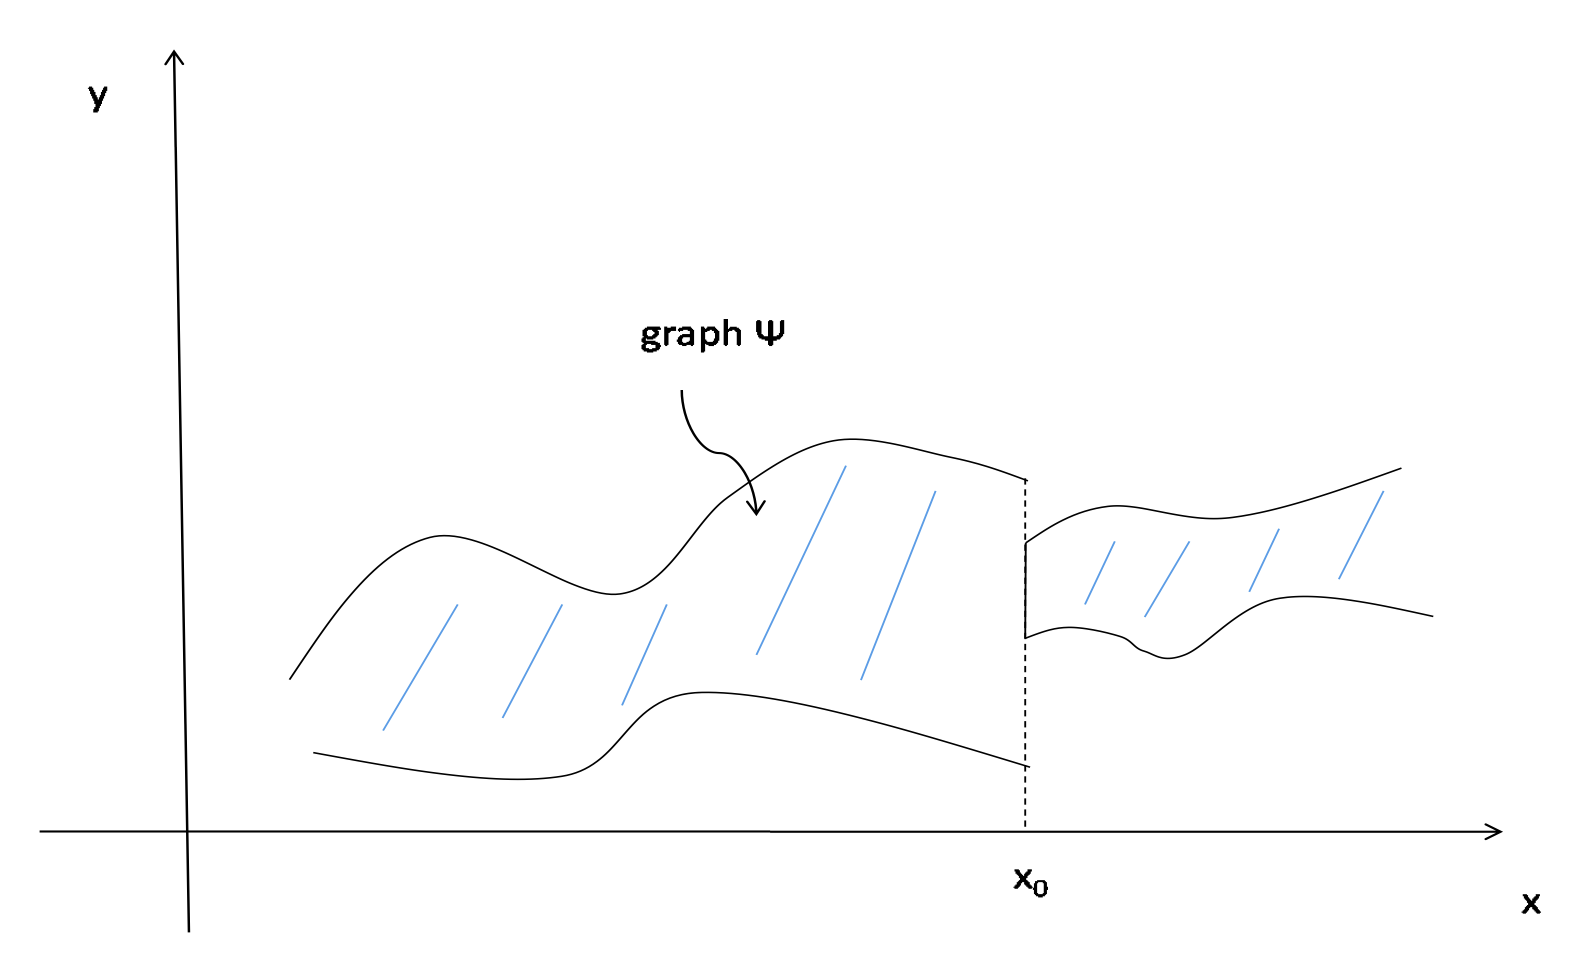
\includegraphics[scale=0.2]{uhc.png}
    \caption{The correspondence $\Psi$ “implodes in the limit” at $x_0$. $\Psi$ is not upper hemicontinuous at $x_0$.}
    \label{}
\end{figure}\end{center}

\begin{center}\begin{figure}[htbp]
    \centering
    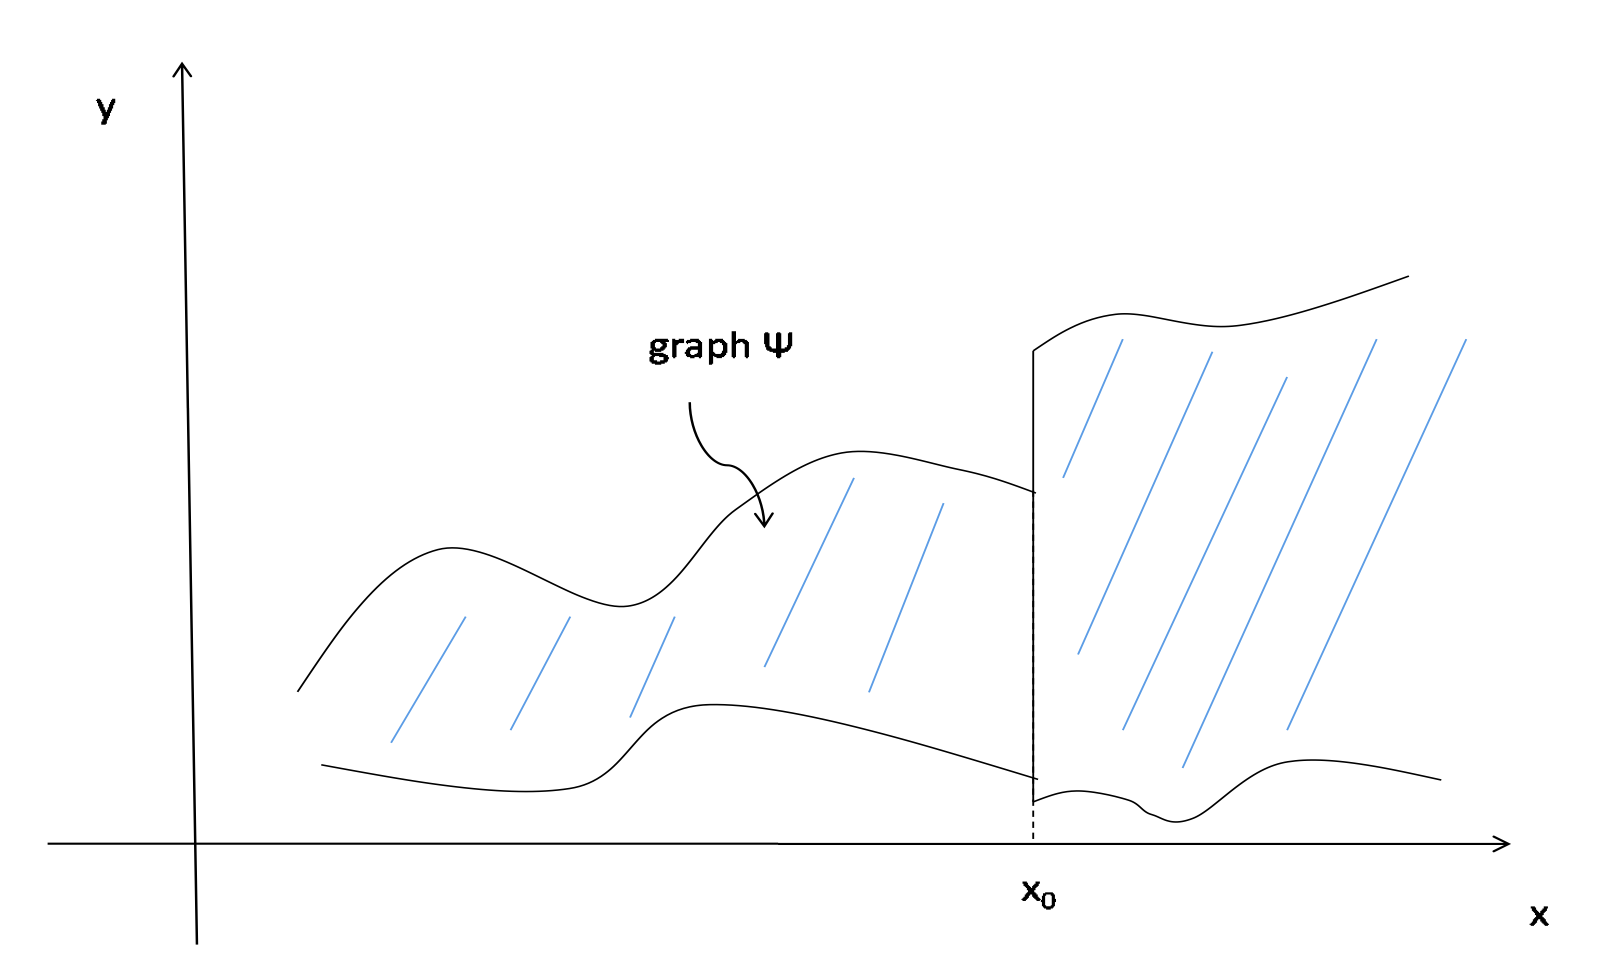
\includegraphics[scale=0.2]{lhc.png}
    \caption{The correspondence $\Psi$ “explodes in the limit” at $x_0$. $\Psi$ is not lower hemicontinuous at $x_0$.}
    \label{}
\end{figure}\end{center}

\subsection{Theorem: $\Psi(x)=\{f(x)\}$ is uhc $\Leftrightarrow$ $f$ is continuous}
\begin{theorem}[$\Psi(x)=\{f(x)\}$ is uhc $\Leftrightarrow$ $f$ is continuous]
    Let $X \subseteq \mathbb{E}^n$, $Y \subseteq \mathbb{E}^m$ and $f : X \rightarrow Y$. Let $\Psi : X \rightarrow  2^Y$ be defined by $\Psi(x) = \{f(x)\}$ for all $x \in X$. Then $\Psi$ is \textbf{uhc} \underline{if and only if} $f$ is \textbf{continuous}.
\end{theorem}


\subsection{Berge's Maximum Theorem: $v(y)=\max_{x\in\Gamma(y)}f(x,y)$ is continuous; $\{x:f(x,y)=v(y)\}$ is uhc with non-empty compact values}
\begin{theorem}[Berge's Maximum Theorem]
    Let $X \subseteq \mathbb{R}^n$ and $Y \subseteq \mathbb{R}^m$. Consider the function $f : X \times Y \rightarrow \mathbb{R}$ and the correspondence $\Gamma : Y \rightarrow 2^X$. Define $v(y) = \max_{x\in\Gamma(y)} f(x, y)$ and $Ω(y) = \argmax_{x\in\Gamma(y)} f(x, y)=\{x:f(x,y)=v(y)\}$. Suppose $f$ and $\Gamma$ are continuous, and that $\Gamma$ has non-empty compact values. Show that v is continuous and $\Omega$ is uhc with non-empty compact values.
\end{theorem}




\section{Graph of Correspondence}
An alternative notion of continuity looks instead at properties of the graph of the correspondence.
\begin{definition}[Graph of Correspondence]
    \normalfont
    The \textbf{graph} of a correspondence $\Psi : X \rightarrow 2^Y$ is the set
    $$\textnormal{graph}\Psi=\{(x,y)\in X\times Y:y\in\Psi(x)\}$$
\end{definition}

\subsection{Closed Graph}
By the definition of continuous function $f:\mathbb{R}^n \rightarrow \mathbb{R}$,  each convergent sequence $\{(x_n, y_n)\}$ in graph $f$ converges to a point $(x, y)$ in graph $f$, that is, graph $f$ is closed.

\begin{definition}[Closed Graph]
    \normalfont
    Let $X\subseteq \mathbb{E}^n$, $Y\subseteq \mathbb{E}^m$. A correspondence $\Psi: X \rightarrow 2^Y$ has closed graph if its graph is a closed subset of $X \times Y$, that is, if for any sequences $\{x_n\} \subseteq X$ and $\{y_n\} \subseteq Y$ such that $x_n \rightarrow x \in X$, $y_n \rightarrow y \in Y$ and $y_n \in \Psi(x_n)$ for each $n$, then $y \in \Psi(x)$.
\end{definition}
\begin{example}
    Consider the correspondence $\Psi(x)=\left\{\begin{matrix}
        \{\frac{1}{x}\},&\textnormal{ if }x\in(0,1]\\
        \{0\},&\textnormal{ if }x=0
    \end{matrix}\right.$ ("implode in the limit")\\
    Let $V = (-0.1, 0.1)$. Then $\Psi(0) = \{0\} \subseteq V$, but no matter how close $x$ is to $0$, $\Psi(x)=\{\frac{1}{x}\}\nsubseteq V$, so $\Psi$ is not uhc at $0$. However, note that $\Psi$ has closed graph.
\end{example}

\section{Closed-valued and Compact-valued Correspondences}
\begin{definition}[Closed-valued and Compact-valued Correspondences]
    \normalfont
    Given a correspondence $\Psi : X \rightarrow 2^Y$,
    \begin{enumerate}
        \item $\Psi$ is \textbf{closed-valued} if $\Psi(x)$ is a closed subset of $Y$ for all $x$;
        \item $\Psi$ is \textbf{compact-valued} if $\Psi(x)$ is compact for all $x$.
    \end{enumerate}
\end{definition}

\subsection{Closed-valued, uhc and Closed Graph}
For closed-valued correspondences these concepts can be more tightly connected. A closed-valued and upper hemicontinuous correspondence must have closed graph. For a closed-valued correspondence with a compact range, upper hemicontinuity is equivalent to closed graph.

\begin{theorem}[Properties]
    Let $X\subseteq \mathbb{E}^n$, $Y\subseteq \mathbb{E}^m$, and $\Psi: X \rightarrow 2^Y$.
    \begin{enumerate}[(i).]
        \item $\Psi$ is \textbf{closed-valued} and \textbf{uhc} $\Rightarrow$ $\Psi$ has \textbf{closed graph}.
        \item $\Psi$ is \textbf{closed-valued} and \textbf{uhc} $\Leftrightarrow$ $\Psi$ has \textbf{closed graph}. (If $Y$ is \textbf{compact})
        \item If $\Psi$ has \textbf{closed graph} and there is an \textbf{open set} $W$ with $x_0 \in W$ and a \textbf{compact set} $Z$ such that $x \in W \cap X \Rightarrow \Psi(x) \subseteq Z$, then $\Psi$ is \textbf{uhc} at $x_0$.
    \end{enumerate}
\end{theorem}



\subsection{Theorem: compact-valued, uhs correspondence of compact set is compact}
\begin{theorem}\label{thm:compact-valued, uhs correspondence of compact set is compact}
    Let $X$ be a compact set and $\Psi : X \rightarrow 2^X$ be a non-empty, compact-valued upper-hemicontinuous correspondence. If $C \subseteq X$ is compact, then $\Psi(C)$ is compact.
\end{theorem}
\begin{proof}
    Given the compact-valued $\Psi$, we can have an open cover of $\Psi(C)$, $\{U_\lambda:\lambda\in\Lambda\}$. So $\forall x\in C$, there exists $U_{l(x)},l(x)\in\Lambda$ such that $U_{l(x)}$ is an open cover of $\Psi(x)$.

    Consider a $c\in C$. Since $\Psi$ is uhs and $\Psi(c)\subseteq U_{l(c)}$, there exists open set $V_c$ s.t. $c\in V_c$ and $\Psi(x)\subseteq U_{l(c)}, \forall x\in V_c\cap C$.

    $\{V_c:c\in C\}$ is an open cover of $C$. Because $C$ is compact, there is a finite subcover $\{V_{c_i}: i=1,...,m\},m\in \mathbb{N}$, where $\{c_i:i=1,...,m\}\subseteq C$.

    Because $\Psi(x)\subseteq U_{l(c_i)}, \forall x\in V_{c_i}\cap C$ and $\{V_{c_i}: i=1,...,m\},m\in \mathbb{N}$ is a open cover for $C$, we can infer $\{U_{l(c_i)}:i=1,...,m\}$ is a finite subcover of $\{U_{l(c)}:c\in C\}$ for $\Psi(C)$. Hence, $C$ is compact.
\end{proof}

\section{Fixed Points for Correspondences \small{(@ Lec 13 of ECON 204)}}
\subsection{Definition}
\begin{definition}[Fixed Points for Correspondences]
    \normalfont
    Let $X$ be nonempty and $\psi : X \rightarrow 2^X$ be a correspondence. A point $x^* \in X$ is a fixed point of $\psi$ if $x^* \in \psi(x^*)$.
\end{definition}
\begin{note}
    We only need $x^*$ to be in $\psi(x^*)$, not $\{x^*\} = \psi(x^*)$. That is, $\psi$ need not be single-valued at $x^*$. So $x^*$ can be a fixed point of $\psi$ but there may be other elements of $\psi(x^*)$ different from $x^*$.
\end{note}



\subsection{Kakutani's Fixed Point Theorem: Existence of a Fixed Point}
\begin{theorem}[Kakutani's Fixed Point Theorem]
    Let $X \subseteq \mathbb{R}^n$ be a non-empty, \textbf{compact}, \textbf{convex} set and $\psi : X \rightarrow 2^X$ be an \textbf{upper hemi-continuous} correspondence with non-empty, \textbf{compact}, \textbf{convex} values. Then $\psi$ has a fixed point in $X$.
\end{theorem}


\subsection{Theorem: $\exists$ compact set $C = \cap_{i=0}^\infty \Psi^i(X)$ s.t. $\Psi(C)=C$}
\begin{theorem}
    Let $(X, d)$ be a compact metric space and let $\Psi(x) : X \rightarrow 2^X$ be a upper-hemicontinuous, compact-valued correspondence, such that $\Psi(x)$ is non-empty for every $x \in X$. There exists a compact non-empty subset $C\subseteq X$, such that $\Psi(C) \equiv \cup_{x\in C}\Psi(x) = C$.
\end{theorem}
\begin{proof}
    Let's construct a sequence $\{C_n\}$ such that $C_0=X$, $C_1=\Psi(C_0)$, ..., $C_n=\Psi(C_{n-1}),...$ We claim that $C=\cap_{i=0}^\infty C_i$ is a non-empty compact set and satisfies $\Psi(C)=C$.
    \begin{enumerate}
        \item Because we can infer $\Psi(X_1)\subseteq \Psi(X_2)$ if $X_1\subseteq X_2$, $X=C_0\supseteq C_1 \Rightarrow C_1=\Psi(C_0)\supseteq C_2=\Psi(C_1)$,...., so $C_0\supseteq C_1\supseteq \cdots C_n\supseteq \cdots$. Hence, $C$ is not empty.
        \item Because $X$ is compact, by the theorem \ref{thm:compact-valued, uhs correspondence of compact set is compact}, we can infer $C_n$ is compact for all $n$. Then, $C_n$ is closed for all $n$, so $C$ is closed. Because $C$ is a closed set of compact set $X$, $C$ is compact.
        \item $C\subseteq C_n,\forall n \Rightarrow \Psi(C)\subseteq \Psi(C_n),\forall n \Rightarrow \Psi(C)\subseteq C$
        \item Assume $C\subseteq \Psi(C)$ doesn't hold, that is $\exists y\in C$ s.t. $y\notin \Psi(C)$. Because $y\in C$ and $C_0\supseteq C_1\supseteq \cdots C_n\supseteq \cdots$, there exists $k\in C_n$ for all $n$ s.t. $y\in\Psi(k)$. $k\in \cap_{i=1}^\infty C_i=C$, so $\Psi(k)\subseteq \Psi(C)$, which contradicts to $y\notin \Psi(C)$. Hence, $C\subseteq \Psi(C)$.
    \end{enumerate}
    All in all the claim "$C=\cap_{i=0}^\infty C_i$ is a non-empty compact set and satisfies $\Psi(C)=C$" is proved.
\end{proof}













\chapter{Differential Equations \small{(@ Lec 14/15 of ECON 204)}}
\section{Initial Value Problem}
\subsection{Initial Value Problem}
\begin{definition}[Differential Equation]
    \normalfont
    A \textbf{differential equation} is an equation of the form $y'(t)=F(y(t), t)$.
\end{definition}
where $F : U \rightarrow \mathbb{R}^n$ and $U$ is an open subset of $\mathbb{R}^n\times \mathbb{R}$.

\begin{definition}[Initial Value Problem]
    \normalfont
    \begin{enumerate}
        \item An initial value problem is a differential equation combined with an initial condition $$y(t_0)=y_0$$
        where $(y_0,t_0)\in U$
        \item A solution of the initial value problem is a differentiable function $y : (a, b) \rightarrow \mathbb{R}^n$ such that $t_0 \in (a, b)$, $y(t_0) = y_0$ and, for all $t \in (a, b)$, $y'(t)=F(y(t), t)$.
        \item The general solution of the differential equation is the family of all solutions for all initial values $(y_0, t_0) \in U$.
    \end{enumerate}
\end{definition}

\subsection{Theorem: Initial Value Problem, Continuous $\rightarrow$ Existence; Lipschitz $\rightarrow$ Uniqueness}
\begin{theorem}[Initial Value Problem, Continuous $\rightarrow$ Existence; Lipschitz $\rightarrow$ Uniqueness]
    Consider the initial value problem $$y'(t)=F(y(t), t),\ y(t_0)=y_0$$
    $U$ is an open subset of $\mathbb{R}^n\times \mathbb{R}$ containing $(y_0,t_0)$.
    \begin{enumerate}
        \item Suppose $F : U \rightarrow \mathbb{R}^n$ is continuous. Then the initial value problem has a solution.
        \item If, in addition, F is Lipschitz in $y$ on $U$
        
        (i.e. there is a constant K such that for all $(y,t),(\hat{y},t)\in U$, $|F(y,t)-F(\hat{y},t)|\leq K|y-\hat{y}|$),
        
        then there is an interval $(a, b)$ containing $t_0$ such that the solution is unique on $(a, b)$.
    \end{enumerate}
\end{theorem}

\begin{example}
    Consider the initial value problem $$y'(t) = 1 + y^2(t), y(0) = 0$$
    Here, we have $F(y, t) = 1 + y^2$ which is Lipschitz in $y$ over $U = V \times \mathbb{R}$, provided that $V$ is bounded, but not over all of $\mathbb{R} \times \mathbb{R}$. The theorem tells us that the initial value problem has a unique solution over some interval of $t$, $(a, b)$, with $0 \in (a, b)$.\\
    We can find $y(t)=\tan t$ is a unique solution in $(a,b)\subsetneq (-\frac{\pi}{2},\frac{\pi}{2})$ with $a<0,b>0$.
\end{example}

\begin{example}
    Consider the initial value problem $$y'(t) = 2\sqrt{|y|}, y(0) = 0$$
    As $F(y)=2\sqrt{|y|}$ is not locally Lipschitz in $y$ at $y = 0$, we can find for all $\alpha\geq 0$, $$y_\alpha(t)=\left\{\begin{matrix}
        0,&t\leq \alpha\\
        (t-\alpha)^2,&t\geq \alpha
    \end{matrix}\right.$$ is a solution of the initial value problem, which is not unique.
\end{example}

\section{Autonomous Differential Equation}
\subsection{Autonomous Differential Equation}
\begin{definition}[Autonomous Differential Equation]
    \normalfont
    An \textbf{autonomous differential equation} is a differential equation of the form $y'(t) = F(y(t))$
    where $F : \mathbb{R}^n \rightarrow \mathbb{R}^n$ depends on t only through the value of $y(t)$.

    A \textbf{stationary point} of an autonomous differential equation is a point $y_s \in \mathbb{R}^n$ such that $F(y_s) = 0$.
\end{definition}

We study the qualitative properties of autonomous differential equations by looking for stationary points. The constant function
$$
y(t)=y_s
$$
is a solution (and the unique solution when $F$ is Lipschitz) of the initial value problem
$$
y^{\prime}=F(y), y\left(t_0\right)=y_s
$$
If $F$ is $C^2$, then Taylor's Theorem implies that near a stationary point $y_s$,
$$
\begin{aligned}
F\left(y_s+h\right) & =F\left(y_s\right)+D F\left(y_s\right) h+O\left(|h|^2\right) \\
& =D F\left(y_s\right) h+O\left(|h|^2\right)
\end{aligned}
$$
Thus, when we are sufficiently close to the stationary point, the solutions of the autonomous differential equation are closely approximated by the solutions of the linear differential equation
$$
y^{\prime}=\left(y-y_s\right)^{\prime}=D F\left(y_s\right)\left(y-y_s\right)
$$
Thus, we study solutions of linear differential equations, using linear algebra. For this we first recall the formulation of complex exponentials, which are central in the general solution of linear differential equations.

\subsection{Complex Exponentials}
By the Taylor series, $e^x=\sum_{k=0}^\infty\frac{x^k}{k!}$. If $x=a+ib\in \mathbb{C}$, $a,b\in \mathbb{R}$, we have
\begin{equation}
    \begin{aligned}
        e^{x}&=e^{a+ib}=e^a e^{ib}\\
        &=e^a\left(\sum_{k=0}^\infty(-1)^k\frac{b^{2k}}{(2k)!}+i\sum_{k=0}^\infty(-1)^k\frac{b^{2k+1}}{(2k+1)!}\right)\\
        &=e^a(\cos b + i\sin b)
    \end{aligned}
    \nonumber
\end{equation}
Hence,
\begin{enumerate}
    \item If $a < 0$, then $e^{tx} \rightarrow  0$ as $t \rightarrow \infty$.
    \item If $a > 0$, then $|e^{tx}| \rightarrow  \infty$ as $t \rightarrow \infty$.
    \item If $a = 0$, then $|e^{tx}| \rightarrow  1$ for all $t\in \mathbb{R}$.
\end{enumerate}

\subsection{Solutions of Simple Case: $y'(t)=ay(t)$}
\begin{proposition}[Simple Case]
    Given $y'(t)=ay(t)$, we have
    \begin{equation}
        \begin{aligned}
            y(t)=c e^{at}, c\in \mathbb{R}^*
        \end{aligned}
        \nonumber
    \end{equation}
\end{proposition}
\begin{proof}
    \begin{equation}
        \begin{aligned}
            y'(t)=\frac{dy}{dt}&=a y\\
            \frac{dy}{y}&=a dt\\
            \int \frac{1}{y} dy &= \int a dt\\
            \ln y &= at +c',\ c'\in \mathbb{R}\\
            y(t)&=e^{c'} e^{at}=c e^{at},\ c\in \mathbb{R}^*
        \end{aligned}
        \nonumber
    \end{equation}
\end{proof}
\begin{proposition}[Simple Case with Initial Value]\label{proposition:Simple Case with Initial Value}
    Given initial value $(t_0,y_0)$, $y'(t)=a y(t)$, we have
    \begin{equation}
        \begin{aligned}
            y(t)=y_0 e^{a(t-t_0)}
        \end{aligned}
        \nonumber
    \end{equation}
\end{proposition}

\subsection{Solutions of Special Case: Linear Differential Equations with Constant Coefficients}
Let $M \in \mathbb{R}^{n\times n}$. The linear differential equation $$
y^{\prime}=\left(y-y_s\right)^{\prime}=M\left(y-y_s\right)
$$
has a complete solution in closed form.

The matrix representation $$M=D F\left(y_s\right)$$
need not be symmetric, hence may not be diagonalizable. If $M$ is diagonalizable over $\mathbb{C}$, the complete solution takes the following simple form:

\begin{theorem}[Solutions of Linear Differential Equations with Constant Coefficients]\label{theorem:Solutions of Linear Differential Equations with Constant Coefficients}
    Consider the linear differential equation $$
    y^{\prime}=\left(y-y_s\right)^{\prime}=M\left(y-y_s\right)
    $$
    where M is a real $n\times n$ matrix. Suppose that M can be diagonalized over the complex field $\mathbb{C}$. Let $U$ be the standard basis of $\mathbb{R}^n$ and $V = \{v_1, . . . , v_n\}$ be a basis of (complex) eigenvectors corresponding to the eigenvalues $\lambda_1, . . . , \lambda_n \in \mathbb{C}$ of $M$. Then the solution of the initial value problem is given by
    \begin{equation}
        \begin{aligned}
            y(t)=y_s+P^{-1}\begin{bmatrix}
                e^{\lambda_1(t-t_0)}&0&0&0\\
                0&e^{\lambda_2(t-t_0)}&0&0\\
                \vdots&\vdots&\ddots&\vdots\\
                0&0&0&e^{\lambda_n(t-t_0)}
            \end{bmatrix} P(y(t_0)-y_s)
        \end{aligned}
        \label{Constant Coefficients}
    \end{equation}
    where $P = \textnormal{Mtx}_{V,U}(id)$, and the general complex solution is obtained by allowing $y(t_0)$ to vary over $\mathbb{C}^n$; it has $n$ complex degrees of freedom. The general real solution is obtained by allowing $y(t_0)$ to vary over $\mathbb{R}^n$; it has $n$ real degrees of freedom. Every real solution is a linear combination of the real and imaginary parts of a complex solution. In particular,
    \begin{enumerate}
        \item If the real part of each eigenvalue is less than zero, all solutions converge to $y_s$.
        \item If the real part of each eigenvalue is greater than zero, all solutions diverge from $y_s$ and tend to infinity.
        \item If the real parts of some eigenvalues are less than zero and the real parts of other eigenvalues are greater than zero, solutions follow roughly hyperbolic paths.
        \item If the real parts of all eigenvalues are zero, all solutions follow closed cycles around $y_s$.
    \end{enumerate}
\end{theorem}
\begin{note}
    If one or more of the eigenvalues are complex, each of the three matrices in Equation \ref{Constant Coefficients} will contain complex entries, but the product of the three matrices is real. Thus, if the initial condition $y_0$ is real, Equation \ref{Constant Coefficients} gives us a real solution; indeed, it gives us the unique solution of the initial value problem.
\end{note}

\begin{note}
    Given a fixed time $t_0$, the general real solution is obtained by varying the initial values of $y(t_0)$ over $\mathbb{R}^n$, which provides $n$ real degrees of freedom. You might think that varying $t_0$ provides one additional degree of freedom, but it doesn't. Given any solution satisfying the initial condition $y(t_0) = y_0$, the solution is defined on some interval $(t_0-\delta, t_0+ \delta)$; given $t_1 \in (t_0-\delta, t_0 +\delta)$, let $y_1 = y(t_1)$; then the solution with initial condition $y_1 = y(t_1)$ is the same as the solution with initial condition $y_0 = y(t_0)$. The same holds true for the general complex solution.
\end{note}

\begin{proof}
    Let $P=\textnormal{Mtx}_{V,U}(id)$. Rewrite the differential equation in terms of a new variable $$z=Py$$
    Let $z_s=Py_s$, then we have
    \begin{equation}
        \begin{aligned}
            z-z_s&=P(y-y_s)\\
            (z-z_s)'=z'&=P y'\\
            &=PM(y-y_s)\\
            &=PMP^{-1}(z-z_s)\\
            &=B(z-z_s)
        \end{aligned}
        \nonumber
    \end{equation}
    where $B=\textnormal{diag}(\lambda_1,...,\lambda_n)$.

    Thus, the $i^{th}$ component of $(z(t)-z_s)$ satisfies
    \begin{equation}
        \begin{aligned}
            (z(t)-z_s)'_i&=\lambda_i(z(t)-z_s)_i\\
        \end{aligned}
        \nonumber
    \end{equation}
    by the proposition \ref{proposition:Simple Case with Initial Value}, we have
    \begin{equation}
        \begin{aligned}
            (z(t)-z_s)_i=e^{\lambda_i(t-t_0)}(z(t_0)-z_s)_i
        \end{aligned}
        \nonumber
    \end{equation}
    so,
    \begin{equation}
        \begin{aligned}
            z(t)-z_s&=\begin{bmatrix}
                e^{\lambda_1(t-t_0)}&0&0&0\\
                0&e^{\lambda_2(t-t_0)}&0&0\\
                \vdots&\vdots&\ddots&\vdots\\
                0&0&0&e^{\lambda_n(t-t_0)}
            \end{bmatrix} (z(t_0)-z_s)
        \end{aligned}
        \nonumber
    \end{equation}
    \begin{equation}
        \begin{aligned}
            y(t)-y_s&=P^{-1}\begin{bmatrix}
                e^{\lambda_1(t-t_0)}&0&0&0\\
                0&e^{\lambda_2(t-t_0)}&0&0\\
                \vdots&\vdots&\ddots&\vdots\\
                0&0&0&e^{\lambda_n(t-t_0)}
            \end{bmatrix} (z(t_0)-z_s)\\
            &=P^{-1}\begin{bmatrix}
                e^{\lambda_1(t-t_0)}&0&0&0\\
                0&e^{\lambda_2(t-t_0)}&0&0\\
                \vdots&\vdots&\ddots&\vdots\\
                0&0&0&e^{\lambda_n(t-t_0)}
            \end{bmatrix} P(y(t_0)-y_s)\\
        \end{aligned}
        \nonumber
    \end{equation}
\end{proof}


\subsection{The Form of Real Solutions}
We can determine the form of the real solutions once we know the eigenvalues. In an important special case, we can solve for the solution of the initial value problem without calculating the diagonalization, as in Equation \ref{Constant Coefficients}.
\begin{theorem}
    Consider the differential equation
    $$
    y^{\prime}=\left(y-y_s\right)^{\prime}=M\left(y-y_s\right)
    $$
    Suppose that the matrix $M$ can be diagonalized over $\mathbb{C}$. Let the eigenvalues of $M$ with the correct multiplicity be
    $$
    a_1+i b_1, a_1-i b_1, \ldots, a_m+i b_m, a_m-i b_m, a_{m+1}, \ldots, a_{n-m}
    $$
    Then for each fixed $i=1, \ldots, n$, every real solution is of the form
    $$
    \left(y(t)-y_s\right)_i=\sum_{j=1}^m e^{a_j\left(t-t_0\right)}\left(C_{i j} \cos b_j\left(t-t_0\right)+D_{i j} \sin b_j\left(t-t_0\right)\right)+\sum_{j=m+1}^{n-m} C_{i j} e^{a_j\left(t-t_0\right)}
    $$
    The $n^2$ parameters
    $$
    \left\{C_{i j}: i=1, \ldots, n ; j=1, \ldots, n-m\right\} \cup\left\{D_{i j}: i=1, \ldots, n ; j=1, \ldots, m\right\}
    $$
    have $n$ real degrees of freedom. The parameters are uniquely determined from the $n$ real initial conditions of an initial value problem.
\end{theorem}


\section{Higher Order Differential Equations}
When we consider a differential equation of order $n$ is an equation of the form
\begin{equation}
    \begin{aligned}
        y^{(n)}(t)=F\left(y(t),y'(t),...,y^{n-1}(t),t\right)
    \end{aligned}
    \nonumber
\end{equation}
We can always rewrite
\begin{equation}
    \begin{aligned}
        \bar{y}(t)=\begin{bmatrix}
            y(t)\\y'(t)\\
            \vdots\\y^{n-1}(t)
        \end{bmatrix}
    \end{aligned}
    \nonumber
\end{equation}

\subsection{Second Order Linear Differential Equations}
Consider the second order differential equation $y'' = cy + by'$ with $b, c \in \mathbb{R}$.

Rewrite $\bar{y}(t)=\begin{bmatrix}
    y(t)\\ y'(t)
\end{bmatrix}$, then
\begin{equation}
    \begin{aligned}
        \bar{y}'(t)=\begin{bmatrix}
            y'(t)\\ y''(t)
        \end{bmatrix}=\begin{bmatrix}
            0&1\\
            c&b
        \end{bmatrix}\begin{bmatrix}
            y(t)\\ y'(t)
        \end{bmatrix}=\begin{bmatrix}
            0&1\\
            c&b
        \end{bmatrix}\bar{y}
    \end{aligned}
    \nonumber
\end{equation}
By the Theorem \ref{theorem:Solutions of Linear Differential Equations with Constant Coefficients}, we can now solve it. Specifically, the eigenvalues of $\begin{bmatrix}
    0&1\\
    c&b
\end{bmatrix}$ are $\frac{b\pm\sqrt{b^2+4c}}{2}$.

\begin{example}
    Consider the second order linear differential equation $y''=2y+y'$, we can solve the eigenvalues $\lambda_1=2,\lambda_2=-1$ and eigenvectors $v_1=(1,2), v_2=(1,-1)$. The general solution of $\bar{y}(t)=\begin{bmatrix}
        y(t)\\ y'(t)
    \end{bmatrix}$ can be solved by the Theorem \ref{theorem:Solutions of Linear Differential Equations with Constant Coefficients}.
\end{example}

\section{Inhomogeneous Linear Differential Equations with Nonconstant Coefficients}
Consider the inhomogeneous linear differential equation
\begin{equation}
    \begin{aligned}
        y'=M(t)y+H(t)
    \end{aligned}
    \tag{1}
    \label{Equation 1}
\end{equation}
where $M$ is continuous function from $t$ to the set of $n \times n$ matrices; and $H$ is continuous
function from $t$ to $\mathbb{R}^n$.

\subsection{Theorem: General Solution of Inhomo $=$ General Solution of Homo $+$ Particular Solution of Inhomo}
There is a close relationship between solutions of the \textit{inhomogeneous} linear differential equation \ref{Equation 1} and the associated \textit{homogeneous} linear differential equation
\begin{equation}
    \begin{aligned}
        y'=M(t)y
    \end{aligned}
    \tag{2}
    \label{Equation 2}
\end{equation}

\begin{theorem}[General Solution of Inhomo$=$General Solution of Homo$+$Particular Solution of Inhomo]
    The general solution of the inhomogeneous linear differential equation \ref{Equation 1} is $$y_h+y_p$$
    where $y_h$ is the general solution of the homogeneous linear differential equation \ref{Equation 2} and $y_p$ is any particular solution of the inhomogeneous linear differential equation \ref{Equation 1}.
\end{theorem}
Hence, to find general solution of inhomogeneous equation:
\begin{enumerate}
    \item Find general solution of homogeneous equation;
    \item Find a particular solution of inhomogeneous equation;
    \item Add these to get general solution of inhomogeneous equation
\end{enumerate}




\subsection{Matrix Exponentials Notations}
In analogy with how we define $e^x$ for $x \in \mathbb{R}$, for an $n \times n$ matrix $M$ we define
$$
e^M=\sum_{k=0}^{\infty} \frac{M^k}{k !}=I+M+\frac{M^2}{2}+\cdots
$$
and
$$
e^{t M}=\sum_{k=0}^{\infty} \frac{t^k M^k}{k !}
$$
The matrix exponential satisfies many properties analogous to the exponential function in $\mathbb{R}$ and $\mathbb{C}$. Here are a few of the most important properties, which can be established fairly directly from the definitions above.
\begin{enumerate}[-]
    \item If $D$ is a diagonal matrix with diagonal $d_1, \ldots, d_n$,
    $$
    e^D=\left(\begin{array}{cccc}
    e^{d_1} & 0 & \cdots & 0 \\
    0 & e^{d_2} & \cdots & 0 \\
    \vdots & \vdots & \ddots & \vdots \\
    0 & 0 & \cdots & e^{d_n}
    \end{array}\right)
    $$
    \item $e^{A+B}=e^A e^B$ if $A B=B A$ (this is not necessarily valid for matrices $A$ and $B$ that do not commute)
    \item $e^{P^{-1} A P}=P^{-1} e^A P$\\
    Then, if $M$ is diagonalizable, so $M = P^{-1}DP$ for a diagonal matrix $D$, then $$e^M=P^{-1} e^D P=P^{-1} \left(\begin{array}{cccc}
        e^{d_1} & 0 & \cdots & 0 \\
        0 & e^{d_2} & \cdots & 0 \\
        \vdots & \vdots & \ddots & \vdots \\
        0 & 0 & \cdots & e^{d_n}
        \end{array}\right) P$$
    \item $g(t)=e^{t M}$ is differentiable (in fact $C^{\infty}$) and $g^{\prime}(t)=M e^{t M}$
\end{enumerate}


\subsection{Theorem: Particular Solution of Inhomogeneous Linear Differential Equations with Constant Coefficients (Matrix)}
\begin{theorem}[Particular  Solution with Constant Coefficients (Matrix)]
    Consider the inhomogeneous linear differential equation \ref{Equation 1}, and suppose that $M(t)$ is a constant matrix $M$, independent of $t$. A particular solution of the inhomogeneous linear differential equation \ref{Equation 1}, satisfying the initial condition $y_p(t_0) = y_0$, is given by
    \begin{equation}
        \begin{aligned}
            y_p(t_0)&=e^{(t-t_0)M}y_0+\int_{t_0}^t e^{(t-s)M} H(s) ds
        \end{aligned}
        \tag{3}
        \label{Equation 3}
    \end{equation}
\end{theorem}


\chapter{Big $\mathcal{O}$ and Small $o$ Notation}
\section{Definition}
\begin{definition}["$O$" and "$o$"]
    \normalfont
    \begin{enumerate}
        \item $y = O(|h|^n)$ as $h \rightarrow 0$ -- read “$y$ is big-Oh of $|h|^n$” -- means $\exists K, \delta > 0$ s.t. $|h| < \delta \Rightarrow |y| \leq K|h|^n$
        \item $y = o(|h|^n)$ as $h \rightarrow 0$ -- read “$y$ is little-Oh of $|h|^n$” -- means $\lim_{h \rightarrow 0}\frac{|y|}{|h|^n}=0$
    \end{enumerate}
\end{definition}
\begin{center}
    \fcolorbox{black}{gray!10}{\parbox{.9\linewidth}{\textbf{\underline{Complexity}:}
    \begin{definition}
        A sequence $f(n)$ is $O(1)$ if $\lim_{n \rightarrow \infty}f(n)<\infty$.
    \end{definition}
    
    \begin{definition}
        A sequence $f(n)$ is $O(g(n))$ if $\frac{f(n)}{g(n)}$ is $O(1)$.
    \end{definition}
    
    \begin{definition}
        A sequence $f(n)$ is $o(1)$ if $\lim_{n \rightarrow \infty}\sup f(n)=0$.
    \end{definition}
    
    \begin{definition}
        A sequence $f(n)$ is $o(g(n))$ if $\lim_{n \rightarrow \infty}\sup \frac{f(n)}{g(n)}=0$.
    \end{definition}
    
    \begin{definition}
        A sequence $f(n)$ is \underline{asymptotic} to $g(n)$ if $\lim_{n \rightarrow \infty} \frac{f(n)}{g(n)}=1$. (This is denoted by $f(n)\sim g(n)$ as $a \rightarrow \infty$)
    \end{definition}
    }}
\end{center}
For two scalar functions $f(x)\in \mathbb{R}, g(x)\in \mathbb{R}_+$, where $x\in \mathbb{R}$, we write:
\begin{enumerate}
    \item $f(x)=\mathcal{O}(g(x))$ if $\lim \sup_{x \rightarrow	\infty}\frac{|f(x)|}{g(x)}<\infty$; we say $f$ is dominated by $g$ asymptotically.
    \item $f(x)=\Omega(g(x))$ if $\lim \inf_{x \rightarrow \infty}\frac{|f(x)|}{g(x)}>0$.
    \item $f(x)=\Theta (g(x))$ if $f(x)=\mathcal{O}(g(x))$ and $f(x)=\Omega(g(x))$ both hold.
    \item $f(x)=o(g(x))$ if $\lim \inf_{x \rightarrow \infty}\frac{f(x)}{g(x)}=0$.
\end{enumerate}

\begin{example}
\begin{equation}
    \begin{aligned}
        n^3+n+2=\Omega(1),n^3+n+2=\Omega(n^2)\\
        n^3+n+2=\Theta(n^3)\\
        n^3+n+2=o(n^4)
    \end{aligned}
    \nonumber
\end{equation}
\end{example}

\subsection{Extension}
$f(x)=\mathcal{O}(g(x))$ as $x \rightarrow a$ if $\lim \sup_{x \rightarrow a}\frac{|f(x)|}{g(x)}<\infty$.

\begin{example}
$\varepsilon^2+\varepsilon^3=\mathcal{O}(\varepsilon^2)$ as $\varepsilon \rightarrow 0$
\end{example}




\end{document}